
%% Light Questions used on the
%% NYSED Physics Regents Examination
%%--------------------------------------------------

%% this section contains 148 problems


%% Section June2016
%%--------------------
\element{nysed}{
\begin{question}{June2016-Q16}
    A \SI{5.09e14}{\hertz} electromagnetic wave is traveling through a transparent medium. 
    The main factor that determines the speed of this wave is the:
    \begin{choices}
      \correctchoice{nature of the medium}
        \wrongchoice{amplitude of the wave}
        \wrongchoice{phase of the wave}
        \wrongchoice{distance traveled through the medium}
    \end{choices}
\end{question}
}

\element{nysed}{
\begin{question}{June2016-Q23}
    A beam of monochromatic light ($f=\SI{5.09e14}{\hertz}$) has a wavelength of \SI{589}{\nano\meter} in air. 
    What is the wavelength of this light in Lucite?
    \begin{multicols}{2}
    \begin{choices}
        \wrongchoice{\SI{150}{\nano\meter}}
      \correctchoice{\SI{393}{\nano\meter}}
        \wrongchoice{\SI{589}{\nano\meter}}
        \wrongchoice{\SI{884}{\nano\meter}}
    \end{choices}
    \end{multicols}
\end{question}
}


%% Section June2015
%%--------------------
\element{nysed}{
\begin{question}{June2015-Q08}
    Which characteristic of a light wave must increase as the light wave passes from glass into air?
    \begin{multicols}{2}
    \begin{choices}
        \wrongchoice{amplitude}
        \wrongchoice{frequency}
        \wrongchoice{period}
      \correctchoice{wavelength}
    \end{choices}
    \end{multicols}
\end{question}
}

\element{nysed}{
\begin{question}{June2015-Q23}
    A gamma ray and a microwave traveling in a vacuum have the same:
    \begin{multicols}{2}
    \begin{choices}
        \wrongchoice{frequency}
        \wrongchoice{period}
      \correctchoice{speed}
        \wrongchoice{wavelength}
    \end{choices}
    \end{multicols}
\end{question}
}

\element{nysed}{
\begin{question}{June2015-Q34}
    The diagram below shows a ray of monochromatic light incident on a boundary between air and glass.
    \begin{center}
    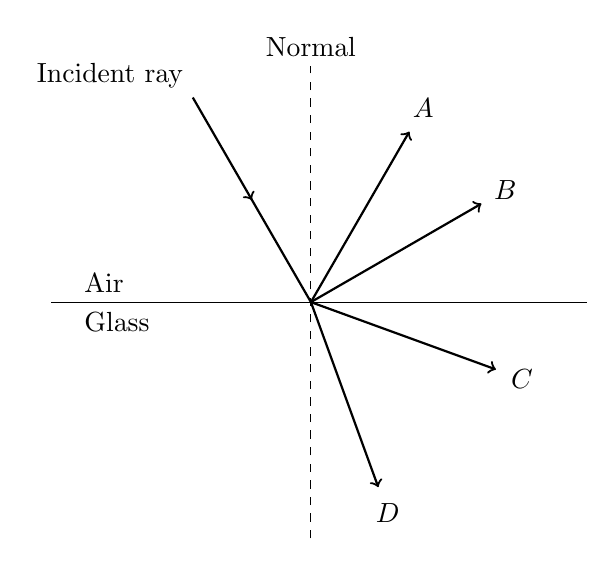
\begin{tikzpicture}
        %% air glass boundary
        \draw (-3.3,0) -- (3.5,0);
        \node[anchor=south west] at (-3,0) {Air};
        \node[anchor=north west] at (-3,0) {Glass};
        \draw[dashed] (0,-3) -- (0,3) node[anchor=south] {Normal};
        %% incident
        \node[anchor=south east] at (120:3) {Incident ray};
        \draw[thick,->] (0,0) -- (120:3) -- ++(300:1.5);
        %% reflected/refracted
        \foreach \x/\y in {60/A,30/B,340/C,290/D}
            \draw[thick,->] (0,0) -- ++(\x:2.5) node[anchor=center,shift={(\x:1em)}] {$\y$};
    \end{tikzpicture}
    \end{center}
    Which ray best represents the path of the reflected light ray?
    \begin{multicols}{4}
    \begin{choices}[o]
      \correctchoice{$A$}
        \wrongchoice{$B$}
        \wrongchoice{$C$}
        \wrongchoice{$D$}
    \end{choices}
    \end{multicols}
\end{question}
}

\element{nysed}{
\begin{question}{June2015-Q46}
    A ray of yellow light ($f=\SI{5.0914}{\hertz}$) travels at a speed of \SI{2.04e8}{\meter\per\second} in:
    \begin{multicols}{2}
    \begin{choices}
        \wrongchoice{ethyl alcohol}
        \wrongchoice{water}
        \wrongchoice{Lucite}
      \correctchoice{glycerol}
    \end{choices}
    \end{multicols}
\end{question}
}

\element{nysed}{
\begin{question}{June2015-Q47}
    A blue-light photon has a wavelength of \SI{4.80e-7}{\meter}.
    What is the energy of the photon?
    \begin{multicols}{2}
    \begin{choices}
        \wrongchoice{\SI{1.86e22}{\joule}}
        \wrongchoice{\SI{1.44e2}{\joule}}
      \correctchoice{\SI{4.14e-19}{\joule}}
        \wrongchoice{\SI{3.18e-26}{\joule}}
    \end{choices}
    \end{multicols}
\end{question}
}


%% Section June2014
%%--------------------
\element{nysed}{
\begin{question}{June2014-Q18}
    As a monochromatic light ray passes from air into water,
        two characteristics of the ray that will \emph{not} change are:
    \begin{choices}
      \correctchoice{frequency and period}
        \wrongchoice{frequency and speed}
        \wrongchoice{wavelength and period}
        \wrongchoice{wavelength and speed}
    \end{choices}
\end{question}
}

\element{nysed}{
\begin{question}{June2014-Q23}
    A beam of light has a wavelength of \SI{4.5e-7}{\meter} in a vacuum.
    The frequency of this light is:
    \begin{multicols}{2}
    \begin{choices}
      \correctchoice{\SI{6.7e14}{\hertz}}
        \wrongchoice{\SI{1.4e2}{\hertz}}
        \wrongchoice{\SI{1.5e-15}{\hertz}}
        \wrongchoice{\SI{4.5e-7}{\hertz}}
    \end{choices}
    \end{multicols}
\end{question}
}

\element{nysed}{
\begin{question}{June2014-Q24}
    When x-ray radiation and infrared radiation are traveling in a vacuum,
        they have the same:
    \begin{choices}
      \correctchoice{speed}
        \wrongchoice{wavelength}
        \wrongchoice{frequency}
        \wrongchoice{energy per photon}
    \end{choices}
\end{question}
}

\element{nysed}{
\begin{question}{June2014-Q41}
    Which graph best represents the relationship between the absolute index of refraction and the speed of light ($f=\SI{5.09e14}{\hertz}$) in various media?
    \begin{multicols}{2}
    \begin{choices} \small
        \AMCboxDimensions{down=-2.5em}
        \correctchoice{
            \begin{tikzpicture}
                \begin{axis}[
                    axis y line=left, 
                    axis x line=bottom, 
                    axis line style={->},
                    xlabel={speed of light},
                    xtick=\empty,
                    ylabel={index of refraction},
                    ytick=\empty,
                    xmin=0,xmax=11,
                    ymin=0,ymax=11,
                    width=\columnwidth,
                ]
                \addplot[line width=1pt,samples=20,domain=0:10]{10/x};
                \end{axis}
            \end{tikzpicture}
        }
        \wrongchoice{
            \begin{tikzpicture}
                \begin{axis}[
                    axis y line=left, 
                    axis x line=bottom, 
                    axis line style={->},
                    xlabel={speed of light},
                    xtick=\empty,
                    ylabel={index of refraction},
                    ytick=\empty,
                    xmin=0,xmax=11,
                    ymin=0,ymax=11,
                    width=\columnwidth,
                ]
                \addplot[line width=1pt,samples=40,domain=0:10]{3.16*sqrt(x)};
                \end{axis}
            \end{tikzpicture}
        }
        \wrongchoice{
            \begin{tikzpicture}
                \begin{axis}[
                    axis y line=left, 
                    axis x line=bottom, 
                    axis line style={->},
                    xlabel={speed of light},
                    xtick=\empty,
                    ylabel={index of refraction},
                    ytick=\empty,
                    xmin=0,xmax=11,
                    ymin=0,ymax=11,
                    width=\columnwidth,
                ]
                \addplot[line width=1pt,samples=20,domain=0:10]{0.1*x*x};
                \end{axis}
            \end{tikzpicture}
        }
        \wrongchoice{
            \begin{tikzpicture}
                \begin{axis}[
                    axis y line=left, 
                    axis x line=bottom, 
                    axis line style={->},
                    xlabel={speed of light},
                    xtick=\empty,
                    ylabel={index of refraction},
                    ytick=\empty,
                    xmin=0,xmax=11,
                    ymin=0,ymax=11,
                    width=\columnwidth,
                ]
                \addplot[line width=1pt,samples=20,domain=0:10]{x};
                \end{axis}
            \end{tikzpicture}
        }
    \end{choices}
    \end{multicols}
\end{question}
}

\element{nysed}{
\begin{question}{June2014-Q46}
    Which graph best represents the relationship between photon energy and photon wavelength?
    \begin{multicols}{2}
    \begin{choices}
        \AMCboxDimensions{down=-2.0em}
        \correctchoice{
            \begin{tikzpicture}
                \begin{axis}[
                    axis y line=left, 
                    axis x line=bottom, 
                    axis line style={->},
                    xlabel={wavelength},
                    xtick=\empty,
                    ylabel={photon energy},
                    ytick=\empty,
                    xmin=0,xmax=11,
                    ymin=0,ymax=11,
                    width=\columnwidth,
                ]
                \addplot[line width=1pt,samples=20,domain=0:10]{10/x};
                \end{axis}
            \end{tikzpicture}
        }
        \wrongchoice{
            \begin{tikzpicture}
                \begin{axis}[
                    axis y line=left, 
                    axis x line=bottom, 
                    axis line style={->},
                    xlabel={wavelength},
                    xtick=\empty,
                    ylabel={photon energy},
                    ytick=\empty,
                    xmin=0,xmax=11,
                    ymin=0,ymax=11,
                    width=\columnwidth,
                ]
                \addplot[line width=1pt,samples=40,domain=0:10]{x};
                \end{axis}
            \end{tikzpicture}
        }
        \wrongchoice{
            \begin{tikzpicture}
                \begin{axis}[
                    axis y line=left, 
                    axis x line=bottom, 
                    axis line style={->},
                    xlabel={wavelength},
                    xtick=\empty,
                    ylabel={photon energy},
                    ytick=\empty,
                    xmin=0,xmax=11,
                    ymin=0,ymax=11,
                    width=\columnwidth,
                ]
                \addplot[line width=1pt,samples=20,domain=0:10]{0.1*x*x};
                \end{axis}
            \end{tikzpicture}
        }
        \wrongchoice{
            \begin{tikzpicture}
                \begin{axis}[
                    axis y line=left, 
                    axis x line=bottom, 
                    axis line style={->},
                    xlabel={wavelength},
                    xtick=\empty,
                    ylabel={photon energy},
                    ytick=\empty,
                    xmin=0,xmax=11,
                    ymin=0,ymax=11,
                    width=\columnwidth,
                ]
                \addplot[line width=1pt,samples=20,domain=0:10]{8};
                \end{axis}
            \end{tikzpicture}
        }
    \end{choices}
    \end{multicols}
\end{question}
}

\element{nysed}{
\begin{question}{June2014-Q49}
    When a ray of light traveling in water reaches a boundary with air,
        part of the light ray is reflected and part is refracted.
    Which ray diagram best represents the paths of the reflected and refracted light rays?
    \begin{multicols}{2}
    \begin{choices}
        \AMCboxDimensions{down=-1.5cm}
        \correctchoice{
            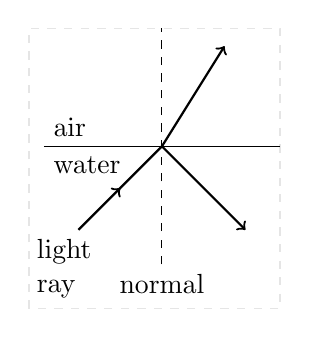
\begin{tikzpicture}[scale=0.75]
                \draw[dashed,white!90!black] (-2.25,-2.75) rectangle (2,2);
                %% axis
                \draw (-2,0) -- (2,0);
                \draw[dashed] (0,-2) -- (0,2);
                %% labels
                \node[anchor=south west] at (-2,0) {air};
                \node[anchor=north west] at (-2,0) {water};
                \node[anchor=north] at (0,-2) {normal};
                \node[anchor=north,text width=3em] at (225:2) {light ray};
                %% incoming
                \draw[thick,->] (0,0) -- ++(225:2) -- ++(45:1);
                %% outgoing
                \draw[thick,->] (0,0) -- ++(58:2);
                \draw[thick,->] (0,0) -- ++(315:2);
            \end{tikzpicture}
        }
        \wrongchoice{
            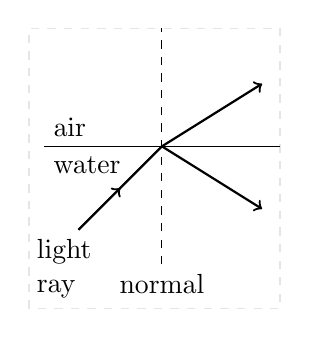
\begin{tikzpicture}[scale=0.75]
                \draw[dashed,white!90!black] (-2.25,-2.75) rectangle (2,2);
                %% axis
                \draw (-2,0) -- (2,0);
                \draw[dashed] (0,-2) -- (0,2);
                %% labels
                \node[anchor=south west] at (-2,0) {air};
                \node[anchor=north west] at (-2,0) {water};
                \node[anchor=north] at (0,-2) {normal};
                \node[anchor=north,text width=3em] at (225:2) {light ray};
                %% incoming
                \draw[thick,->] (0,0) -- ++(225:2) -- ++(45:1);
                %% outgoing
                \draw[thick,->] (0,0) -- ++(32.0:2);
                \draw[thick,->] (0,0) -- ++(328:2);
            \end{tikzpicture}
        }
        \wrongchoice{
            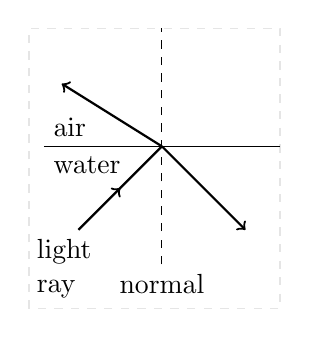
\begin{tikzpicture}[scale=0.75]
                \draw[dashed,white!90!black] (-2.25,-2.75) rectangle (2,2);
                %% axis
                \draw (-2,0) -- (2,0);
                \draw[dashed] (0,-2) -- (0,2);
                %% labels
                \node[anchor=south west] at (-2,0) {air};
                \node[anchor=north west] at (-2,0) {water};
                \node[anchor=north] at (0,-2) {normal};
                \node[anchor=north,text width=3em] at (225:2) {light ray};
                %% incoming
                \draw[thick,->] (0,0) -- ++(225:2) -- ++(45:1);
                %% outgoing
                \draw[thick,->] (0,0) -- ++(148:2);
                \draw[thick,->] (0,0) -- ++(315:2);
            \end{tikzpicture}
        }
        \wrongchoice{
            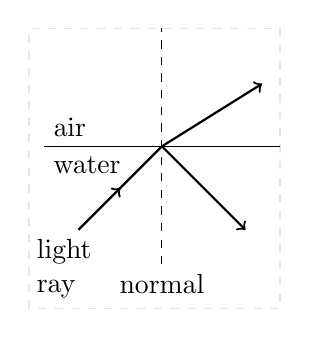
\begin{tikzpicture}[scale=0.75]
                \draw[dashed,white!90!black] (-2.25,-2.75) rectangle (2,2);
                %% axis
                \draw (-2,0) -- (2,0);
                \draw[dashed] (0,-2) -- (0,2);
                %% labels
                \node[anchor=south west] at (-2,0) {air};
                \node[anchor=north west] at (-2,0) {water};
                \node[anchor=north] at (0,-2) {normal};
                \node[anchor=north,text width=3em] at (225:2) {light ray};
                %% incoming
                \draw[thick,->] (0,0) -- ++(225:2) -- ++(45:1);
                %% outgoing
                \draw[thick,->] (0,0) -- ++(32:2);
                \draw[thick,->] (0,0) -- ++(315:2);
            \end{tikzpicture}
        }
    \end{choices}
    \end{multicols}
\end{question}
}


%% Section June2013
%%--------------------
\element{nysed}{
\begin{question}{June2013-Q16}
    Which statement describes a characteristic common to all electromagnetic waves and mechanical waves?
    \begin{choices}
        \wrongchoice{Both types of waves travel at the same speed.}
        \wrongchoice{Both types of waves require a material medium for propagation.}
        \wrongchoice{Both types of waves propagate in a vacuum.}
      \correctchoice{Both types of waves transfer energy}
    \end{choices}
\end{question}
}

\element{nysed}{
\begin{question}{June2013-Q17}
    An electromagnetic wave is produces by charged particles vibrating at a rate of \num{3.9e8} vibrations per second.
    The electromagnetic wave is classified as:
    \begin{multicols}{2}
    \begin{choices}
      \correctchoice{a radio wave}
        \wrongchoice{an infrared wave}
        \wrongchoice{an x-ray}
        \wrongchoice{visible light}
    \end{choices}
    \end{multicols}
\end{question}
}


%% Section June2012
%%--------------------
\element{nysed}{
\begin{question}{June2012-Q27}
    A monochromatic beam of light has a frequency of \SI{7.67e14}{\hertz}.
    What is the energy of a photon of this light?
    \begin{multicols}{2}
    \begin{choices}
        \wrongchoice{\SI{2.59e-40}{\joule}}
        \wrongchoice{\SI{6.92e-31}{\joule}}
      \correctchoice{\SI{5.10e-19}{\joule}}
        \wrongchoice{\SI{3.90e-7}{\joule}}
    \end{choices}
    \end{multicols}
\end{question}
}

\element{nysed}{
\begin{question}{June2012-Q49}
    A ray of light ($f=\SI{5.09e14}{\hertz}$) travels through various substances.
    Which graph best represents the relationship between the absolute index of refraction of these substances and the corresponding speed of light in these substances?
    \begin{multicols}{2}
    \begin{choices} \small
        \AMCboxDimensions{down=-2.5em}
        \correctchoice{
            \begin{tikzpicture}
                \begin{axis}[
                    axis y line=left, 
                    axis x line=bottom, 
                    axis line style={->},
                    xlabel={index of refraction},
                    xtick=\empty,
                    ylabel={speed of light},
                    ytick=\empty,
                    xmin=0,xmax=11,
                    ymin=0,ymax=11,
                    width=\columnwidth,
                ]
                \addplot[line width=1pt,samples=40,domain=0:10]{10/x};
                \end{axis}
            \end{tikzpicture}
        }
        \wrongchoice{
            \begin{tikzpicture}
                \begin{axis}[
                    axis y line=left, 
                    axis x line=bottom, 
                    axis line style={->},
                    xlabel={index of refraction},
                    xtick=\empty,
                    ylabel={speed},
                    ytick=\empty,
                    xmin=0,xmax=11,
                    ymin=0,ymax=11,
                    width=\columnwidth,
                ]
                \addplot[line width=1pt,samples=20,domain=0:10]{sqrt(10)*sqrt(x)};
                \end{axis}
            \end{tikzpicture}
        }
        \wrongchoice{
            \begin{tikzpicture}
                \begin{axis}[
                    axis y line=left, 
                    axis x line=bottom, 
                    axis line style={->},
                    xlabel={index of refraction},
                    xtick=\empty,
                    ylabel={speed of light},
                    ytick=\empty,
                    xmin=0,xmax=11,
                    ymin=0,ymax=11,
                    width=\columnwidth,
                ]
                \addplot[line width=1pt,samples=20,domain=0:10]{8};
                \end{axis}
            \end{tikzpicture}
        }
        \wrongchoice{
            \begin{tikzpicture}
                \begin{axis}[
                    axis y line=left, 
                    axis x line=bottom, 
                    axis line style={->},
                    xlabel={index of refraction},
                    xtick=\empty,
                    ylabel={speed of light},
                    ytick=\empty,
                    xmin=0,xmax=11,
                    ymin=0,ymax=11,
                    width=\columnwidth,
                ]
                \addplot[line width=1pt,samples=20,domain=0:10]{x};
                \end{axis}
            \end{tikzpicture}
        }
    \end{choices}
    \end{multicols}
\end{question}
}


%% Section June2011
%%--------------------


%% Section June2010
%%--------------------
\element{nysed}{
\begin{question}{June2010-Q27}
    A ray of monochromatic yellow light ($f=\SI{5.09e14}{\hertz}$) passes from water through flint glass and into medium $X$, as shown below.
    \begin{center}
    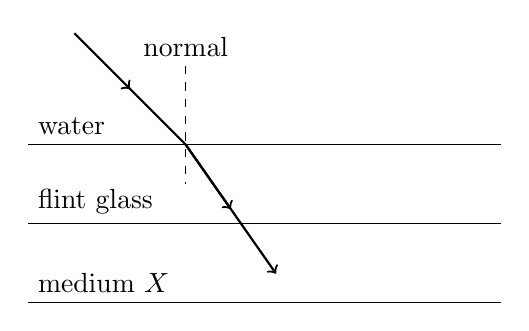
\begin{tikzpicture}
        %% Boundaries
        \draw (-3,2) -- (3,2) node[pos=0,anchor=south west] {water};
        \draw (-3,1) -- (3,1) node[pos=0,anchor=south west] {flint glass};
        \draw (-3,0) -- (3,0) node[pos=0,anchor=south west] {medium $X$};
        %% normal
        \draw[dashed] (-1,3) -- (-1,1.5) node[pos=0,anchor=south] {normal};
        %% light ray
        \draw[thick,->] (-1,2) -- ++ (135:2) -- ++(315:1);
        \draw[thick,->] (-1,2) -- ++ (305:1);
        \draw[thick,->] (-1,2) -- ++ (305:2);
    \end{tikzpicture}
    \end{center}
    The absolute index of refraction of medium $X$ is:
    \begin{choices}
        \wrongchoice{less than \num{1.33}}
        \wrongchoice{greater than \num{1.33} and less than \num{1.52}}
        \wrongchoice{greater than \num{1.52} and less than \num{1.66}}
      \correctchoice{equal to \num{1.66}}
    \end{choices}
\end{question}
}

\element{nysed}{
\begin{question}{June2010-Q28}
    A light ray traveling in air enters a second medium and its speed slows to \SI{1.71e8}{\meter\per\second}.
    What is the absolute index of refraction of the second medium?
    \begin{multicols}{2}
    \begin{choices}
        \wrongchoice{\num{1.00}}
        \wrongchoice{\num{0.570}}
      \correctchoice{\num{1.75}}
        \wrongchoice{\num{1.94}}
    \end{choices}
    \end{multicols}
\end{question}
}

\element{nysed}{
\begin{question}{June2010-Q30}
    In a vacuum, all electromagnetic waves have the same:
    \begin{multicols}{2}
    \begin{choices}
      \correctchoice{speed}
        \wrongchoice{phase}
        \wrongchoice{frequency}
        \wrongchoice{wavelength}
    \end{choices}
    \end{multicols}
\end{question}
}

\element{nysed}{
\begin{question}{June2010-Q49}
    The diagram below represents a light ray reflecting from a plane mirror.
    \begin{center}
    \begin{tikzpicture}
        %% Light Ray
        \draw[thick,->] (0,0) -- (115:3) -- ++(295:1.5);
        \draw[thick,->] (65:3) -- (0,0) -- (65:1.5);
        %% Angle
        \draw[<->,shorten <=1pt,shorten >=1pt] (180:0.75cm) arc(180:115:0.75cm)
            node[pos=0.5,anchor=east] {\ang{65}};
        %% Mirror
        \draw[pattern=north east lines] (-3,0) rectangle (3,-0.15cm);
        \node[anchor=north] at (0,-0.15cm) {Plane Mirror};
    \end{tikzpicture}
    \end{center}
    %% changed wording
    The angle of reflection, with respect to the normal, for the light ray is:
    \begin{multicols}{4}
    \begin{choices}
      \correctchoice{\ang{25}}
        \wrongchoice{\ang{35}}
        \wrongchoice{\ang{50}}
        \wrongchoice{\ang{65}}
    \end{choices}
    \end{multicols}
\end{question}
}


%% Section June2009
%%--------------------
\element{nysed}{
\begin{question}{June2009-Q23}
    Which color of light has a wavelength of \SI{5.0e-7}{\meter} in air?
    \begin{multicols}{2}
    \begin{choices}
        \wrongchoice{blue}
      \correctchoice{green}
        \wrongchoice{orange}
        \wrongchoice{violet}
    \end{choices}
    \end{multicols}
\end{question}
}

\element{nysed}{
\begin{question}{June2009-Q27}
    The diagram below represents a light ray striking the boundary between air and glass.
    \begin{center}
    \begin{tikzpicture}
        %% Incident and Normal Line
        \draw[thick,->] (0,0) -- ++(150:3) -- ++(330:1.5);
        \draw[dashed,thick] (0:0) -- (90:1.5) node[anchor=south] {Normal};
        %% Angle
        \draw[<->,shorten <=1pt,shorten >=1pt] (180:1.25) arc(180:150:1.24)
            node[pos=0.5,anchor=east] {\ang{30}};
        %% Glass and Air
        \draw[thick] (-3,0) -- (3,0);
        \node[pattern=north east lines,minimum width=6cm,anchor=north] at (0,0) {};
        \node[anchor=south east] at (3,0em) {Air};
        \node[anchor=north east] at (3,-1em) {Glass};
    \end{tikzpicture}
    \end{center}
    What would be the angle between this light ray and its reflected ray?
    \begin{multicols}{4}
    \begin{choices}
        \wrongchoice{\ang{30}}
        \wrongchoice{\ang{60}}
      \correctchoice{\ang{120}}
        \wrongchoice{\ang{150}}
    \end{choices}
    \end{multicols}
\end{question}
}

\element{nysed}{
\begin{question}{June2009-Q28}
    In which way does blue light change as it travels from diamond into crown glass?
    \begin{choices}
        \wrongchoice{Its frequency decreases}
        \wrongchoice{Its frequency increases}
        \wrongchoice{Its speed increases}
      \correctchoice{Its speed decreases}
    \end{choices}
\end{question}
}

\element{nysed}{
\begin{question}{June2009-Q33}
    Which phenomenon provides evidence that light has a wave nature?
    \begin{choices}
        \wrongchoice{emission of light from an energy-level transition in a hydrogen atom}
      \correctchoice{diffraction of light passing through a narrow opening}
        \wrongchoice{absorption of light by a black sheet of paper}
        \wrongchoice{reflection of light from a mirror}
    \end{choices}
\end{question}
}

\element{nysed}{
\begin{question}{June2009-Q44}
    The momentum of a photon, $p$, is given by the equation $p=h/\lambda$ where $h$ is Planck's constant and $\lambda$ is the photon's wavelength.
    Which equation correctly represents the energy of a photon in terms of its momentum?
    \begin{multicols}{2}
    \begin{choices}
        \wrongchoice{$E_{photon} = p h c$}
        \wrongchoice{$E_{photon} = \dfrac{hp}{c}$}
        \wrongchoice{$E_{photon} = \dfrac{p}{c}$}
      \correctchoice{$E_{photon} = p c$}
    \end{choices}
    \end{multicols}
\end{question}
}


%% Section Jan2009
%%--------------------
\element{nysed}{
\begin{question}{Jan2009-Q24}
    Compared to the speed of a sound wave in air,
        the speed of a radio wave in air is:
    \begin{multicols}{3}
    \begin{choices}
        \wrongchoice{less}
      \correctchoice{greater}
        \wrongchoice{the same}
    \end{choices}
    \end{multicols}
\end{question}
}

\element{nysed}{
\begin{question}{Jan2009-Q27}
    Which characteristic is the same for every color of light in a vacuum?
    \begin{multicols}{2}
    \begin{choices}
        \wrongchoice{energy}
        \wrongchoice{frequency}
      \correctchoice{speed}
        \wrongchoice{period}
    \end{choices}
    \end{multicols}
\end{question}
}

\element{nysed}{
\begin{question}{Jan2009-Q28}
    What is the speed of light ($f=\SI{5.09e14}{\hertz}$) in flint glass?
    \begin{multicols}{2}
    \begin{choices}
      \correctchoice{\SI{1.81e8}{\meter\per\second}}
        \wrongchoice{\SI{1.97e8}{\meter\per\second}}
        \wrongchoice{\SI{3.00e8}{\meter\per\second}}
        \wrongchoice{\SI{4.98e8}{\meter\per\second}}
    \end{choices}
    \end{multicols}
\end{question}
}

\element{nysed}{
\begin{question}{Jan2009-Q30}
    A television remote control is used to direct pulses of electromagnetic radiation to a receiver on a television.
    This communication from the remote control to the television illustrates that electromagnetic radiation:
    \begin{choices}
        \wrongchoice{is a longitudinal wave}
        \wrongchoice{posses energy inversely proportional to its frequency}
        \wrongchoice{diffracts and accelerates in air}
      \correctchoice{transfers energy without transferring mass}
    \end{choices}
\end{question}
}

\element{nysed}{
\begin{question}{Jan2009-Q31}
    A wave of constant wavelength diffracts as it passes through an opening in a barrier.
    As the size of the opening is increased,
        the diffraction effects:
    \begin{choices}
      \correctchoice{decrease}
        \wrongchoice{increase}
        \wrongchoice{remain the same}
    \end{choices}
\end{question}
}

\element{nysed}{
\begin{question}{Jan2009-Q46}
    A ray of light ($f=\SI{5.09e14}{\hertz}$) traveling in air incident at an angle of \ang{40} on an air-crown glass interface as shown below.
    \begin{center}
    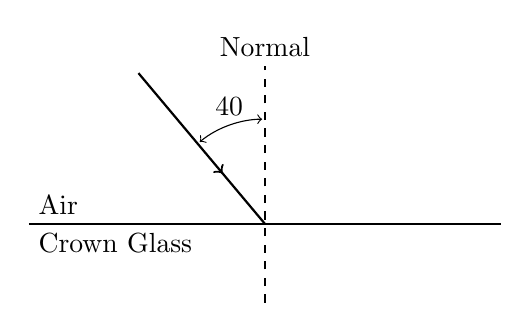
\begin{tikzpicture}
        %% Incident and Normal Line
        \draw[thick,->] (0,0) -- ++(130:2.5) -- ++(310:1.66);
        \draw[<->,shorten >=1pt,shorten <=1pt] (90:1.33) arc (90:130:1.33)
            node[pos=0.5,anchor=south] {\ang{40}};
        \draw[dashed,thick] (0,-1) -- (0,2) node[anchor=south] {Normal};
        %% Glass and Air
        \draw[thick] (-3,0) -- (3,0);
        \node[anchor=south west] at (-3,-0.00cm) {Air};
        \node[anchor=north west] at (-3,-0.00cm) {Crown Glass};
    \end{tikzpicture}
    \end{center}
    What is the angle of refraction for this light ray?
    \begin{multicols}{4}
    \begin{choices}
      \correctchoice{\ang{25}}
        \wrongchoice{\ang{37}}
        \wrongchoice{\ang{40}}
        \wrongchoice{\ang{78}}
    \end{choices}
    \end{multicols}
\end{question}
}


%% Section June2008
%%--------------------
\element{nysed}{
\begin{question}{June2008-Q26}
    An electromagnetic AM-band radio wave could have a wavelength of:
    \begin{multicols}{2}
    \begin{choices}
        \wrongchoice{\SI{0.005}{\meter}}
        \wrongchoice{\SI{5}{\meter}}
      \correctchoice{\SI{500}{\meter}}
        \wrongchoice{\SI{5 000 000}{\meter}}
    \end{choices}
    \end{multicols}
\end{question}
}

\element{nysed}{
\begin{question}{June2008-Q28}
    When light enters a new medium and is refracted,
        there must be a change in the light wave's:
    \begin{multicols}{2}
    \begin{choices}
        \wrongchoice{color}
        \wrongchoice{frequency}
        \wrongchoice{period}
      \correctchoice{speed}
    \end{choices}
    \end{multicols}
\end{question}
}

\element{nysed}{
\begin{question}{June2008-Q29}
    The speed of light in a piece of plastic is \SI{2.00e8}{\meter\per\second}.
    What is the absolute index of refraction of this plastic?
    \begin{multicols}{4}
    \begin{choices}
        \wrongchoice{1.00}
        \wrongchoice{0.670}
        \wrongchoice{1.33}
      \correctchoice{1.50}
    \end{choices}
    \end{multicols}
\end{question}
}

\element{nysed}{
\begin{question}{June2008-Q49}
    Which graph best represents the relationship between photon energy and photon frequency?
    \begin{multicols}{2}
    \begin{choices}
        \AMCboxDimensions{down=-2.5em}
        \correctchoice{
            \begin{tikzpicture}
                \begin{axis}[
                    axis y line=left, 
                    axis x line=bottom, 
                    axis line style={->},
                    xlabel={frequency},
                    xtick=\empty,
                    ylabel={photon energy},
                    ytick=\empty,
                    xmin=0,xmax=11,
                    ymin=0,ymax=11,
                    width=\columnwidth,
                ]
                \addplot[line width=1pt,samples=40,domain=0:10]{x};
                \end{axis}
            \end{tikzpicture}
        }
        \wrongchoice{
            \begin{tikzpicture}
                \begin{axis}[
                    axis y line=left, 
                    axis x line=bottom, 
                    axis line style={->},
                    xlabel={frequency},
                    xtick=\empty,
                    ylabel={photon energy},
                    ytick=\empty,
                    xmin=0,xmax=11,
                    ymin=0,ymax=11,
                    width=\columnwidth,
                ]
                \addplot[line width=1pt,samples=20,domain=0:10]{10-x};
                \end{axis}
            \end{tikzpicture}
        }
        \wrongchoice{
            \begin{tikzpicture}
                \begin{axis}[
                    axis y line=left, 
                    axis x line=bottom, 
                    axis line style={->},
                    xlabel={frequency},
                    xtick=\empty,
                    ylabel={photon energy},
                    ytick=\empty,
                    xmin=0,xmax=11,
                    ymin=0,ymax=11,
                    width=\columnwidth,
                ]
                \addplot[line width=1pt,samples=20,domain=0:10]{10/x};
                \end{axis}
            \end{tikzpicture}
        }
        \wrongchoice{
            \begin{tikzpicture}
                \begin{axis}[
                    axis y line=left, 
                    axis x line=bottom, 
                    axis line style={->},
                    xlabel={frequency},
                    xtick=\empty,
                    ylabel={photon energy},
                    ytick=\empty,
                    xmin=0,xmax=11,
                    ymin=0,ymax=11,
                    width=\columnwidth,
                ]
                \addplot[line width=1pt,samples=20,domain=0:10]{8};
                \end{axis}
            \end{tikzpicture}
        }
    \end{choices}
    \end{multicols}
\end{question}
}


%% Section Jan2008
%%--------------------
\element{nysed}{
\begin{question}{Jan2008-Q26}
    An electromagnetic wave traveling through a vacuum has a wavelength of \SI{1.5e-1}{\meter}.
    What is the period of this electromagnetic wave?
    \begin{multicols}{2}
    \begin{choices}
      \correctchoice{\SI{5.0e-10}{\second}}
        \wrongchoice{\SI{1.5e-1}{\second}}
        \wrongchoice{\SI{4.5e-1}{\second}}
        \wrongchoice{\SI{2.0e9}{\second}}
    \end{choices}
    \end{multicols}
\end{question}
}

\element{nysed}{
\begin{question}{Jan2008-Q27}
    A ray of light ($f=\SI{5.09e14}{\hertz}$) traveling in air strikes a block of sodium chloride at an angle of incidence of \ang{30}.
    What is the angle of refraction for the light ray in the sodium chloride?
    \begin{multicols}{4}
    \begin{choices}
      \correctchoice{\ang{19}}
        \wrongchoice{\ang{25}}
        \wrongchoice{\ang{40}}
        \wrongchoice{\ang{49}}
    \end{choices}
    \end{multicols}
\end{question}
}

\element{nysed}{
\begin{question}{Jan2008-Q28}
    The speed of a ray of light traveling through a substance having an absolute index of refraction of \num{1.1} is:
    \begin{multicols}{2}
    \begin{choices}
        \wrongchoice{\SI{1.1e8}{\meter\per\second}}
      \correctchoice{\SI{2.7e8}{\meter\per\second}}
        \wrongchoice{\SI{3.0e8}{\meter\per\second}}
        \wrongchoice{\SI{3.3e8}{\meter\per\second}}
    \end{choices}
    \end{multicols}
\end{question}
}

\element{nysed}{
\begin{question}{Jan2008-Q33}
    A variable-frequency light source emits a series of photons.
    As the frequency of the photon increases,
        what happens to the energy and wavelength of the photon?
    \begin{choices}
        \wrongchoice{The energy decreases and the wavelength decreases.}
        \wrongchoice{The energy decreases and the wavelength increases.}
      \correctchoice{The energy increases and the wavelength decreases.}
        \wrongchoice{The energy increases and the wavelength increases.}
    \end{choices}
\end{question}
}

\element{nysed}{
\begin{question}{Jan2008-Q49}
    Which diagram best represents the behavior of a ray of monochromatic light in air incident on a block of crown glass?
    \begin{choices}
        \AMCboxDimensions{down=-1.5cm}
        \wrongchoice{
            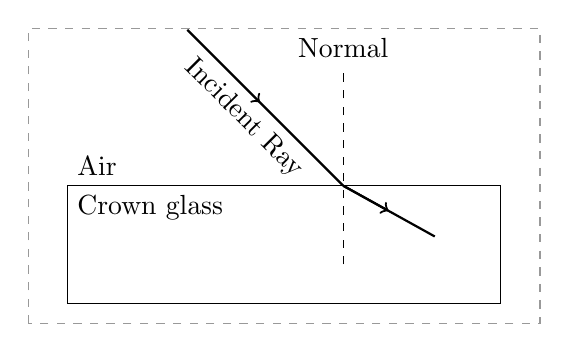
\begin{tikzpicture}
                \draw[dashed,white!60!black] (-4,-1.75) rectangle (2.5,2);
                %% crown glass
                \draw (-3.5,-1.5) rectangle (2,0);
                \node[anchor=north west] at (-3.5,0) {Crown glass};
                %% air
                \node[anchor=south west] at (-3.5,0) {Air};
                \draw[dashed] (0,-1) -- (0,1.5) node[anchor=south] {Normal};
                %% incident
                \draw[thick,->] (0,0) -- ++(135:2.8) -- ++(315:1.3) node[anchor=north,rotate=-45] {Incident Ray};
                %% complement refracted
                \draw[thick,->] (0,0) -- ++(331:0.66);
                \draw[thick] (0,0) -- ++(331:1.33);
            \end{tikzpicture}
        }
        \wrongchoice{
            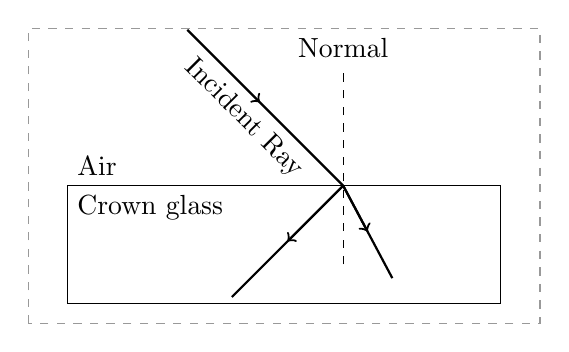
\begin{tikzpicture}
                \draw[dashed,white!60!black] (-4,-1.75) rectangle (2.5,2);
                %% crown glass
                \draw (-3.5,-1.5) rectangle (2,0);
                \node[anchor=north west] at (-3.5,0) {Crown glass};
                %% air
                \node[anchor=south west] at (-3.5,0) {Air};
                \draw[dashed] (0,-1) -- (0,1.5) node[anchor=south] {Normal};
                %% incident
                \draw[thick,->] (0,0) -- ++(135:2.8) -- ++(315:1.3) node[anchor=north,rotate=-45] {Incident Ray};
                %% reverse reflected
                \draw[thick,->] (0,0) -- ++(225:1);
                \draw[thick] (0,0) -- ++(225:2);
                %% refracted
                \draw[thick,->] (0,0) -- ++(298:0.66);
                \draw[thick] (0,0) -- ++(298:1.33);
            \end{tikzpicture}
        }
        \wrongchoice{
            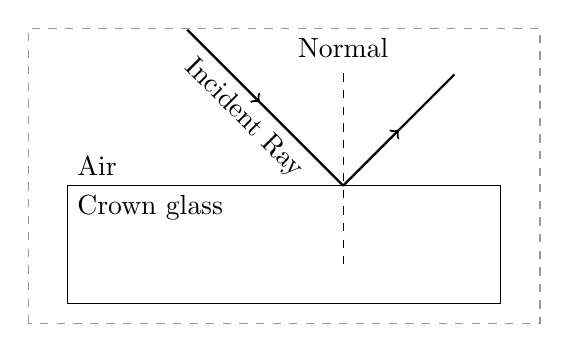
\begin{tikzpicture}
                \draw[dashed,white!60!black] (-4,-1.75) rectangle (2.5,2);
                %% crown glass
                \draw (-3.5,-1.5) rectangle (2,0);
                \node[anchor=north west] at (-3.5,0) {Crown glass};
                %% air
                \node[anchor=south west] at (-3.5,0) {Air};
                \draw[dashed] (0,-1) -- (0,1.5) node[anchor=south] {Normal};
                %% incident
                \draw[thick,->] (0,0) -- ++(135:2.8) -- ++(315:1.3) node[anchor=north,rotate=-45] {Incident Ray};
                %% reflected
                \draw[thick,->] (0,0) -- ++(45:1);
                \draw[thick] (0,0) -- ++(45:2);
            \end{tikzpicture}
        }
        %% ANS is D
        \correctchoice{
            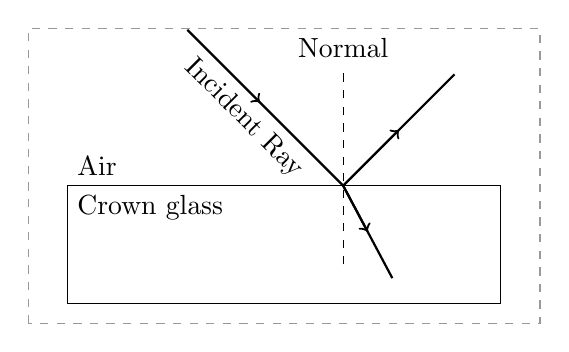
\begin{tikzpicture}
                \draw[dashed,white!60!black] (-4,-1.75) rectangle (2.5,2);
                %% crown glass
                \draw (-3.5,-1.5) rectangle (2,0);
                \node[anchor=north west] at (-3.5,0) {Crown glass};
                %% air
                \node[anchor=south west] at (-3.5,0) {Air};
                \draw[dashed] (0,-1) -- (0,1.5) node[anchor=south] {Normal};
                %% incident
                \draw[thick,->] (0,0) -- ++(135:2.8) -- ++(315:1.3) node[anchor=north,rotate=-45] {Incident Ray};
                %% reflected
                \draw[thick,->] (0,0) -- ++(45:1);
                \draw[thick] (0,0) -- ++(45:2);
                %% refracted
                \draw[thick,->] (0,0) -- ++(298:0.66);
                \draw[thick] (0,0) -- ++(298:1.33);
            \end{tikzpicture}
        }
    \end{choices}
\end{question}
}


%% Section June2007
%%--------------------
\element{nysed}{
\begin{question}{June2007-Q21}
    As yellow light ($f=\SI{5.09e14}{\hertz}$) travels from zircon into diamond, the speed of light:
    \begin{choices}
      \correctchoice{decreases}
        \wrongchoice{increases}
        \wrongchoice{remains the same}
    \end{choices}
\end{question}
}

\element{nysed}{
\begin{question}{June2007-Q24}
    What is the period of a \SI{60}{\hertz} electromagnetic wave traveling at \SI{3.0e8}{\meter\per\second}?
    \begin{multicols}{2}
    \begin{choices}
      \correctchoice{\SI{1.7e-2}{\second}}
        \wrongchoice{\SI{2.0e-7}{\second}}
        \wrongchoice{\SI{6.0e1}{\second}}
        \wrongchoice{\SI{5.0e6}{\second}}
    \end{choices}
    \end{multicols}
\end{question}
}

\element{nysed}{
\begin{question}{June2007-Q26}
    A microwave and an x-ray are traveling in a vacuum.
    Compared to the wavelength and period of the microwave,
        the x-ray has a wavelength that is:
    \begin{choices}
      \correctchoice{shorter and a period that is longer}
        \wrongchoice{shorter and a period that is shorter}
        \wrongchoice{longer and a period that is longer}
        \wrongchoice{longer and a period that is shorter}
    \end{choices}
\end{question}
}

\element{nysed}{
\begin{question}{June2007-Q29}
    A beam of monochromatic light approaches a barrier having four openings, $A$, $B$, $C$, and $D$, of difference sizes as shown below.
    \begin{center}
    \begin{tikzpicture}
        %% NOTE: TODO: draw tikz
    \end{tikzpicture}
    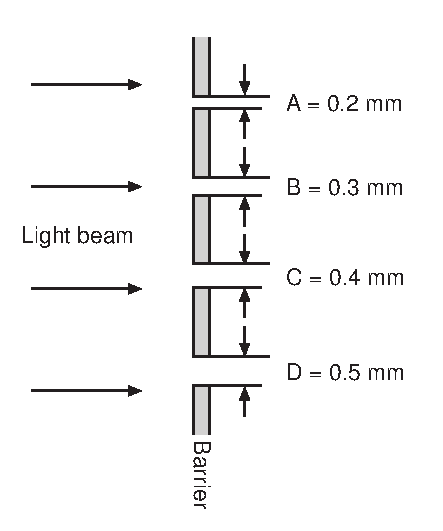
\includegraphics[keepaspectratio,scale=0.75]{June2007-Q29}
    \end{center}
    Which opening will cause the greatest diffraction?
    \begin{multicols}{4}
    \begin{choices}[o]
      \correctchoice{$A$}
        \wrongchoice{$B$}
        \wrongchoice{$C$}
        \wrongchoice{$D$}
    \end{choices}
    \end{multicols}
\end{question}
}

\element{nysed}{
\begin{question}{June2007-Q34}
    Light demonstrates the characteristics of:
    \begin{choices}
      \correctchoice{both particles and waves}
        \wrongchoice{neither particles and waves}
        \wrongchoice{particles, only}
        \wrongchoice{waves, only}
    \end{choices}
\end{question}
}

\element{nysed}{
\begin{question}{June2007-Q46}
    The slope of a graph of photon energy versus photon frequency represents:
    \begin{choices}
      \correctchoice{Planck's constant}
        \wrongchoice{the mass of a photon}
        \wrongchoice{the speed of light}
        \wrongchoice{the speed of light squared}
    \end{choices}
\end{question}
}

%% Section Jan2007
%%--------------------
\element{nysed}{
\begin{question}{Jan2007-Q23}
    What is the speed of a radio wave in a vacuum?
    \begin{multicols}{2}
    \begin{choices}
      \correctchoice{\SI{3.00e8}{\meter\per\second}}
        \wrongchoice{\SI{1.13e3}{\meter\per\second}}
        \wrongchoice{\SI{0}{\meter\per\second}}
        \wrongchoice{\SI{3.31e2}{\meter\per\second}}
    \end{choices}
    \end{multicols}
\end{question}
}

\element{nysed}{
\begin{question}{Jan2007-Q26}
    A straight glass rod appears to bend when placed in a beaker of water,
        as shown in the diagram below.
    \begin{center}
        %% I like this diagram
        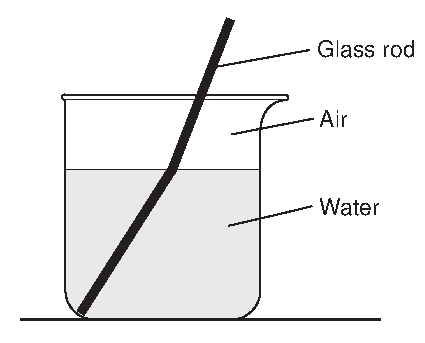
\includegraphics[keepaspectratio,scale=1.00]{Jan2007-Q26}
    \end{center}
    What is the best explanation for this phenomenon?
    \begin{choices}
      \correctchoice{Light is refracted as it cross the air-water interface.}
        \wrongchoice{Light is reflected at the air-water interface.}
        \wrongchoice{The water is warmer than the air.}
        \wrongchoice{Light travels faster in water than in air.}
    \end{choices}
\end{question}
}

\element{nysed}{
\begin{question}{Jan2007-Q27}
    What happens to the speed and frequency of a light ray when it passes from air into water?
    \begin{choices}
      \correctchoice{The speed decreases and the frequency remains the same.}
        \wrongchoice{The speed decreases and the frequency increases.}
        \wrongchoice{The speed increases and the frequency remains the same.}
        \wrongchoice{The speed increases and the frequency increases.}
    \end{choices}
\end{question}
}

\element{nysed}{
\begin{question}{Jan2007-Q32}
    A photon of light traveling through space with a wavelength of \SI{6.0e07}{\meter} has an energy of:
    \begin{multicols}{2}
    \begin{choices}
      \correctchoice{\SI{3.3e-19}{\joule}}
        \wrongchoice{\SI{4.0e-40}{\joule}}
        \wrongchoice{\SI{5.4e10}{\joule}}
        \wrongchoice{\SI{5.0e14}{\joule}}
    \end{choices}
    \end{multicols}
\end{question}
}

\element{nysed}{
\begin{question}{Jan2007-Q48}
    Which wavelength is in the infrared range of electromagnetic spectrum?
    \begin{multicols}{2}
    \begin{choices}
      \correctchoice{\SI{100}{\micro\meter}}
        \wrongchoice{\SI{100}{\meter}}
        \wrongchoice{\SI{100}{\nano\meter}}
        \wrongchoice{\SI{100}{\milli\meter}}
    \end{choices}
    \end{multicols}
\end{question}
}

\element{nysed}{
\begin{question}{Jan2007-Q50}
    What is the wavelength of a light ray with frequency \SI{5.09e14}{\hertz} as it travels through Lucite?
    \begin{multicols}{2}
    \begin{choices}
      \correctchoice{\SI{3.93e-7}{\meter}}
        \wrongchoice{\SI{4.89e-7}{\meter}}
        \wrongchoice{\SI{3.39e14}{\meter}}
        \wrongchoice{\SI{7.64e14}{\meter}}
    \end{choices}
    \end{multicols}
\end{question}
}


%% Section June2006
%%--------------------
\element{nysed}{
\begin{question}{June2006-Q17}
    Radio waves are propagated through the interaction of:
    \begin{choices}
      \correctchoice{electric and magnetic fields}
        \wrongchoice{nuclear and electric fields}
        \wrongchoice{gravitational and magnetic fields}
        \wrongchoice{gravitational and electric fields}
    \end{choices}
\end{question}
}

\element{nysed}{
\begin{question}{June2006-Q27}
    Electromagnetic radiation having a wavelength of \SI{1.3e-7}{\meter} would be classified as:
    \begin{multicols}{2}
    \begin{choices}
      \correctchoice{ultraviolet}
        \wrongchoice{infrared}
        \wrongchoice{orange}
        \wrongchoice{blue}
    \end{choices}
    \end{multicols}
\end{question}
}

\element{nysed}{
\begin{question}{June2006-Q29}
    Which diagram best represents the path taken by a ray of monochromatic light as it passes from air through the material shown?
    \begin{multicols}{2}
    \begin{choices}[o]\small
        \AMCboxDimensions{down=-1.5cm}
        %% fling glass = 1.66
        %% water = 1.33
        %% air = 1.00
        \wrongchoice{
            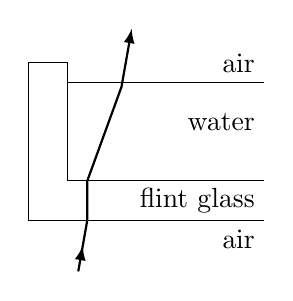
\begin{tikzpicture}
                %% air
                \node[anchor=south east] at (3,1.75) {air};
                %% water
                \draw (0.5,1.75) -- (3,1.75);
                \node[anchor=east] at (3,1.25) {water};
                %% flint glass
                \draw (3,0) -- (0,0) -- (0,2) -- (0.5,2) -- (0.5,0.5) -- (3,0.5);
                \node[anchor=east] at (3,0.25) {flint glass};
                %% air
                \node[anchor=north east] at (3,0) {air};
                %% ray
                \draw[thick,-latex] (0.75,0) -- ++(260:0.66) -- ++(80:0.33);
                \draw[thick,-latex] (0.75,0) -- ++(90:{0.5/sin(90)}) -- ++(70:{1.25/sin(80)}) -- ++(80:0.75);
            \end{tikzpicture}
        }
        \correctchoice{
            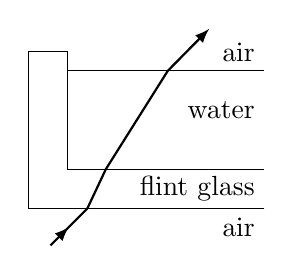
\begin{tikzpicture}
                %% air
                \node[anchor=south east] at (3,1.75) {air};
                %% water
                \draw (0.5,1.75) -- (3,1.75);
                \node[anchor=east] at (3,1.25) {water};
                %% flint glass
                \draw (3,0) -- (0,0) -- (0,2) -- (0.5,2) -- (0.5,0.5) -- (3,0.5);
                \node[anchor=east] at (3,0.25) {flint glass};
                %% air
                \node[anchor=north east] at (3,0) {air};
                %% ray (calculated correct)
                \draw[thick,-latex] (0.75,0) -- ++(225:0.66) -- ++(45:0.33);
                \draw[thick,-latex] (0.75,0) -- ++(64.8:{0.5/sin(64.8)}) -- ++(57.8:{1.25/sin(57.8)}) -- ++(45.4:0.75);
            \end{tikzpicture}
        }
        \wrongchoice{
            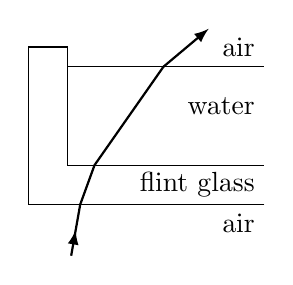
\begin{tikzpicture}
                %% air
                \node[anchor=south east] at (3,1.75) {air};
                %% water
                \draw (0.5,1.75) -- (3,1.75);
                \node[anchor=east] at (3,1.25) {water};
                %% flint glass
                \draw (3,0) -- (0,0) -- (0,2) -- (0.5,2) -- (0.5,0.5) -- (3,0.5);
                \node[anchor=east] at (3,0.25) {flint glass};
                %% air
                \node[anchor=north east] at (3,0) {air};
                %% ray
                \draw[thick,-latex] (0.66,0) -- ++(260:0.66) -- ++(80:0.33);
                \draw[thick,-latex] (0.66,0) -- ++(70:{0.5/sin(70)}) -- ++(55:{1.25/sin(55)}) -- ++(40:0.75);
            \end{tikzpicture}
        }
        \wrongchoice{
            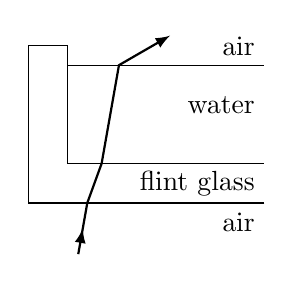
\begin{tikzpicture}
                %% air
                \node[anchor=south east] at (3,1.75) {air};
                %% water
                \draw (0.5,1.75) -- (3,1.75);
                \node[anchor=east] at (3,1.25) {water};
                %% flint glass
                \draw (3,0) -- (0,0) -- (0,2) -- (0.5,2) -- (0.5,0.5) -- (3,0.5);
                \node[anchor=east] at (3,0.25) {flint glass};
                %% air
                \node[anchor=north east] at (3,0) {air};
                %% ray
                \draw[thick,-latex] (0.75,0) -- ++(260:0.66) -- ++(80:0.33);
                \draw[thick,-latex] (0.75,0) -- ++(70:{0.5/sin(70)}) -- ++(80:{1.25/sin(80)}) -- ++(30:0.75);
            \end{tikzpicture}
        }
    \end{choices}
    \end{multicols}
\end{question}
}

\element{nysed}{
\begin{question}{June2006-Q30}
    What is the speed of a ray of light ($f=\SI{5.09e14}{\hertz}$) traveling through a block of sodium chloride?
    \begin{multicols}{2}
    \begin{choices}
      \correctchoice{\SI{1.95e8}{\meter\per\second}}
        \wrongchoice{\SI{4.62e8}{\meter\per\second}}
        \wrongchoice{\SI{3.00e8}{\meter\per\second}}
        \wrongchoice{\SI{1.54e8}{\meter\per\second}}
    \end{choices}
    \end{multicols}
\end{question}
}

\element{nysed}{
\begin{question}{June2006-Q49}
    Compared to the speed of microwaves in a vacuum,
        the speed of x-rays in a vacuum is:
    \begin{multicols}{3}
    \begin{choices}
      \correctchoice{the same}
        \wrongchoice{greater}
        \wrongchoice{less}
    \end{choices}
    \end{multicols}
\end{question}
}


%% Section Jan2006
%%--------------------
\element{nysed}{
\begin{question}{Jan2006-Q31}
    When observed from Earth, the wavelengths of light emitted by a star are shifted toward the red end of the electromagnetic spectrum.
    This redshift occurs because the star is:
    \begin{choices}
      \correctchoice{moving away from Earth}
        \wrongchoice{at rest relative to Earth}
        \wrongchoice{moving toward Earth at decreasing speed}
        \wrongchoice{moving toward Earth at increasing speed}
    \end{choices}
\end{question}
}

\element{nysed}{
\begin{question}{Jan2006-Q34}
    All photons in a vacuum have the same:
    \begin{multicols}{2}
    \begin{choices}
      \correctchoice{speed}
        \wrongchoice{wavelength}
        \wrongchoice{energy}
        \wrongchoice{frequency}
    \end{choices}
    \end{multicols}
\end{question}
}


%% Section June2005
%%--------------------
\element{nysed}{
\begin{question}{June2005-Q25}
    The diagram below shows a ray of light passing from air into glass at an angle of incidence of \ang{0}.
    \begin{center}
    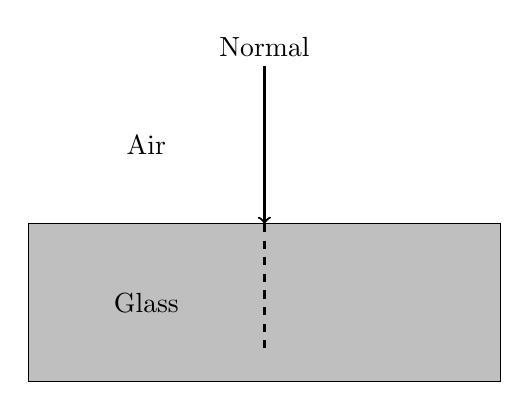
\begin{tikzpicture}
        %% Glass
        \draw[fill=gray!50] (-3,0) rectangle (3,-2);
        \node[anchor=center] at (-1.5,-1) {Glass};
        \node[anchor=center] at (-1.5,1) {Air};
        %% Air and Normal Vector
        \draw[thick,->] (90:2) -- (90:0)
            node[pos=0.0,anchor=south] {Normal};
        \draw[dashed,thick] (0,0) -- (0,-1.66);
    \end{tikzpicture}
    \end{center}
    Which statement best describes the speed and direction of the light ray as it passes into glass?
    \begin{choices}
      \correctchoice{Only speed changes}
        \wrongchoice{Only direction changes}
        \wrongchoice{Both speed and direction change}
        \wrongchoice{Neither speed nor direction change}
    \end{choices}
\end{question}
}

\element{nysed}{
\begin{question}{June2005-Q26}
    A ray of monochromatic light is incident on an air-sodium chloride boundary as shown in the diagram below.
    At the boundary, part of the ray is reflected back into the air and part is refracted as it enters the sodium chloride.
    \begin{center}
    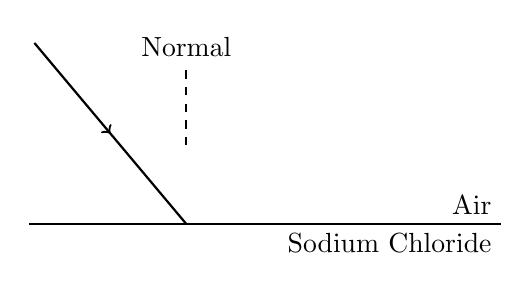
\begin{tikzpicture}
        %% Incident and Normal Line
        \draw[thick,->] (0,0) -- (130:3) -- ++(310:1.5);
        \draw[dashed,thick] (0,1) -- (0,2) node[anchor=south] {Normal};
        %% Glass and Air
        \draw[thick] (-2,0) -- (4,0);
        \node[anchor=south east] at (4,0) {Air};
        \node[anchor=north east] at (4,0) {Sodium Chloride};
    \end{tikzpicture}
    \end{center}
    Compared to the ray's angle of refraction in the sodium chloride,
        the ray's angle of reflection in the air is:
    \begin{multicols}{3}
    \begin{choices}
      \correctchoice{smaller}
        \wrongchoice{larger}
        \wrongchoice{the same}
    \end{choices}
    \end{multicols}
\end{question}
}

\element{nysed}{
\begin{question}{June2005-Q27}
    Which pair of terms best describes light waves traveling from the Sun to the Earth?
    \begin{choices}
      \correctchoice{electromagnetic and transverse}
        \wrongchoice{electromagnetic and longitudinal}
        \wrongchoice{mechanical and transverse}
        \wrongchoice{mechanical and longitudinal}
    \end{choices}
\end{question}
}

\element{nysed}{
\begin{question}{June2005-Q28}
    Which wave characteristic is the same for all types of electromagnetic radiation traveling in a vacuum?
    \begin{multicols}{2}
    \begin{choices}
      \correctchoice{speed}
        \wrongchoice{wavelength}
        \wrongchoice{period}
        \wrongchoice{frequency}
    \end{choices}
    \end{multicols}
\end{question}
}

\element{nysed}{
\begin{question}{June2005-Q30}
    Radio waves diffract around buildings more than light waves do because,
        compared to light waves, radio waves:
    \begin{choices}
      \correctchoice{have a longer wavelength}
        \wrongchoice{have a higher frequency}
        \wrongchoice{move slower}
        \wrongchoice{move faster}
    \end{choices}
\end{question}
}

\element{nysed}{
\begin{question}{June2005-Q42}
    Compared to the period of a wave of red light the period of wave of green light is:
    \begin{multicols}{3}
    \begin{choices}
      \correctchoice{less}
        \wrongchoice{greater}
        \wrongchoice{the same}
    \end{choices}
    \end{multicols}
\end{question}
}


%% Section Jan2005
%%--------------------
\element{nysed}{
\begin{question}{Jan2005-Q12}
    Which form(s) of energy can be transmitted through a vacuum?
    \begin{choices}
      \correctchoice{light, only}
        \wrongchoice{sound, only}
        \wrongchoice{both light and sound}
        \wrongchoice{neither light nor sound}
    \end{choices}
\end{question}
}

\element{nysed}{
\begin{question}{Jan2005-Q15}
    Which quantity is equivalent to the product of the absolute index of refraction of water and the speed of light in water?
    \begin{choices}
      \correctchoice{speed of light in vacuum}
        \wrongchoice{sine of the angle of incidence}
        \wrongchoice{frequency of light in water}
        \wrongchoice{wavelength of light in a vacuum}
    \end{choices}
\end{question}
}

\element{nysed}{
\begin{question}{Jan2005-Q16}
    Radio waves and gamma rays traveling in space have the same:
    \begin{multicols}{2}
    \begin{choices}
      \correctchoice{speed}
        \wrongchoice{frequency}
        \wrongchoice{period}
        \wrongchoice{wavelength}
    \end{choices}
    \end{multicols}
\end{question}
}

\element{nysed}{
\begin{question}{Jan2005-Q17}
    The spreading of a wave into the region behind an obstruction is called:
    \begin{multicols}{2}
    \begin{choices}
      \correctchoice{diffraction}
        \wrongchoice{absorption}
        \wrongchoice{reflection}
        \wrongchoice{refraction}
    \end{choices}
    \end{multicols}
\end{question}
}

\element{nysed}{
\begin{question}{Jan2005-Q41}
    Electrons oscillating with a frequency of \SI{2.0e10}{\hertz} produce electromagnetic waves.
    The waves would be classified as:
    \begin{multicols}{2}
    \begin{choices}
      \correctchoice{microwave}
        \wrongchoice{infrared}
        \wrongchoice{visible}
        \wrongchoice{x-ray}
    \end{choices}
    \end{multicols}
\end{question}
}


%% Section June2004
%%--------------------
\element{nysed}{
\begin{question}{June2004-Q24}
    The energy of a photon is inversely proportional to it:
    \begin{multicols}{2}
    \begin{choices}
      \correctchoice{wavelength}
        \wrongchoice{speed}
        \wrongchoice{frequency}
        \wrongchoice{phase}
    \end{choices}
    \end{multicols}
\end{question}
}

\element{nysed}{
\begin{question}{June2004-Q30}
    A ray of monochromatic light ($f=\SI{5.09e14}{\hertz}$) in air is incident at an angle of \ang{30.} on a boundary with corn oil.
    what is the angle of refraction, to the nearest degree,
        for this light ray in the corn oil?
    \begin{multicols}{4}
    \begin{choices}
      \correctchoice{\ang{20}}
        \wrongchoice{\ang{6}}
        \wrongchoice{\ang{30}}
        \wrongchoice{\ang{47}}
    \end{choices}
    \end{multicols}
\end{question}
}

\element{nysed}{
\begin{question}{June2004-Q31}
    A wave is diffracted as it passes through an opening in a barrier.
    The amount of diffraction that the wave undergoes depends on both the:
    \begin{choices}
      \correctchoice{wavelength of the incident wave and the size of the opening.}
        \wrongchoice{amplitude and frequency of the incident wave.}
        \wrongchoice{wavelength and speed of the incident wave.}
        \wrongchoice{amplitude of the incident wave and the size of the opening.}
    \end{choices}
\end{question}
}

\element{nysed}{
\begin{question}{June2004-Q34}
    A laser beam is directed at the surface of a smooth, calm pond as represented in the diagram below.
    \begin{center}
        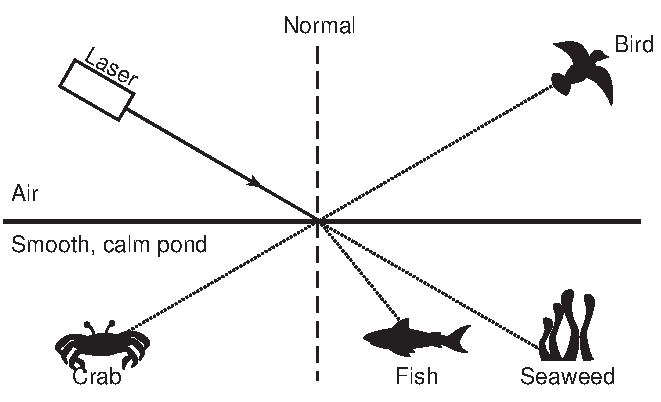
\includegraphics[keepaspectratio,width=\linewidth]{June2004-Q34}
    \end{center}
    \begin{choices}
      \correctchoice{the bird and the fish}
        \wrongchoice{the bird and the seaweed}
        \wrongchoice{the crab and the fish}
        \wrongchoice{the crab and the seaweed}
    \end{choices}
\end{question}
}

\newcommand{\JuneTwentyFourQThirtyNine}{
\begin{tabu}{X[c]X[c]X[c]}
    \toprule
    Photon  & Energy [\si{\joule}]  & Frequency [\si{\hertz}] \\
    \midrule
    $A$     & \num{6.63e-15}        & \num{1.00e19} \\
    $B$     & \num{1.99e-17}        & \num{3.00e16} \\
    $C$     & \num{3.49e-19}        & \num{5.26e14} \\
    $D$     & \num{1.33e-20}        & \num{2.00e13} \\
    $E$     & \num{6.63e-26}        & \num{1.00e8} \\
    \bottomrule
\end{tabu}
}

\element{nysed}{
\begin{question}{June2004-Q39}
    The data table lists the energy and corresponding frequency of five photons.
    \begin{center}
        \JuneTwentyFourQThirtyNine
    \end{center}
    In which part of the electromagnetic spectrum would photon $D$ be found?
    \begin{multicols}{2}
    \begin{choices}
      \correctchoice{infrared}
        \wrongchoice{visible}
        \wrongchoice{x-ray}
        \wrongchoice{ultraviolet}
    \end{choices}
    \end{multicols}
\end{question}
}

\element{nysed}{
\begin{question}{June2004-Q40}
    The data table lists the energy and corresponding frequency of five photons
    \begin{center}
        \JuneTwentyFourQThirtyNine
    \end{center}
    The graph below represents the relationship between the energy and the frequency of photons.
    \begin{center}
    \begin{tikzpicture}
        \begin{axis}[
            axis y line=left, 
            axis x line=bottom, 
            axis line style={->},
            ylabel={energy},
            y unit=\si{\joule},
            ytick=\empty,
            xlabel={frequency},
            x unit=\si{\hertz},
            xtick=\empty,
            ymin=0,ymax=10,
            xmin=0,xmax=10,
            width=0.618\columnwidth,
            height=0.5\columnwidth,
        ]
        \addplot[line width=1pt,domain=0:10]{x};
        \end{axis}
    \end{tikzpicture}
    \end{center}
    The slope of the graph would be:
    \begin{choices}
      \correctchoice{\SI{6.63e-24}{\joule\second}}
        \wrongchoice{\SI{6.67e-11}{\newton\meter\squared\per\kilo\gram\squared}}
        \wrongchoice{\SI{1.60e-19}{\joule}}
        \wrongchoice{\SI{1.60e-19}{\coulomb}}
    \end{choices}
\end{question}
}


%% Section Jan2004
%%--------------------
\element{nysed}{
\begin{question}{Jan2004-Q26}
    How much time does it take light from a flash camera to reach a subject \SI{6.0}{\meter} across a room?
    \begin{multicols}{2}
    \begin{choices}
      \correctchoice{\SI{2.0e-8}{\second}}
        \wrongchoice{\SI{5.0e-9}{\second}}
        \wrongchoice{\SI{5.0e-8}{\second}}
        \wrongchoice{\SI{2.0e-7}{\second}}
    \end{choices}
    \end{multicols}
\end{question}
}

\element{nysed}{
\begin{question}{Jan2004-Q27}
    What happens to the frequency and the speed of an electromagnetic wave as it passes from air into glass?
    \begin{choices}
      \correctchoice{The frequency remains the same and the speed decreases}
        \wrongchoice{The frequency remains the same and the speed increases}
        \wrongchoice{The frequency decreases and the speed increases}
        \wrongchoice{The frequency increases and the speed decreases}
    \end{choices}
\end{question}
}


\element{nysed}{
\begin{question}{Jan2004-Q28}
    Which ray diagram best represents the phenomena of refraction?
    \begin{multicols}{2}
    \begin{choices}[o]
        \AMCboxDimensions{down=-1cm}
        \correctchoice{
            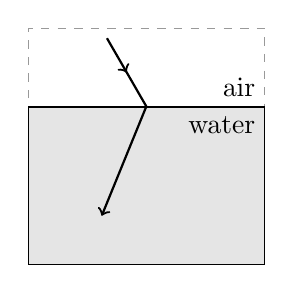
\begin{tikzpicture}
                \draw[dashed,white!60!black] (-1.5,-1) rectangle (1.5,2);
                %% water
                \node[draw,minimum width=3cm,minimum height=2cm,fill=white!90!black] (A) at (0,0) {};
                %% labels
                \node[anchor=north east] at (A.north east) {water};
                \node[anchor=south east] at (A.north east) {air};
                %% Ray
                \draw[thick,->] (A.north) -- ++(120:1) -- ++(300:0.5);
                \draw[thick,->] (A.north) -- ++(247.8:1.5);
            \end{tikzpicture}
        }
        \wrongchoice{
            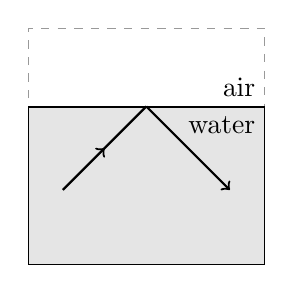
\begin{tikzpicture}
                \draw[dashed,white!60!black] (-1.5,-1) rectangle (1.5,2);
                %% water
                \node[draw,minimum width=3cm,minimum height=2cm,fill=white!90!black] (A) at (0,0) {};
                %% labels
                \node[anchor=north east] at (A.north east) {water};
                \node[anchor=south east] at (A.north east) {air};
                %% Ray
                \draw[thick,->] (A.north) -- ++(225:1.5) -- ++(45:0.75);
                \draw[thick,->] (A.north) -- ++(315:1.5);
            \end{tikzpicture}
        }
        \wrongchoice{
            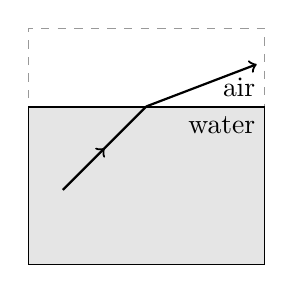
\begin{tikzpicture}
                \draw[dashed,white!60!black] (-1.5,-1) rectangle (1.5,2);
                %% water
                \node[draw,minimum width=3cm,minimum height=2cm,fill=white!90!black] (A) at (0,0) {};
                %% labels
                \node[anchor=north east] at (A.north east) {water};
                \node[anchor=south east] at (A.north east) {air};
                %% Ray
                \draw[thick,->] (A.north) -- ++(225:1.5) -- ++(45:0.75);
                \draw[thick,->] (A.north) -- ++(20.9:1.5);
            \end{tikzpicture}
        }
        \wrongchoice{
            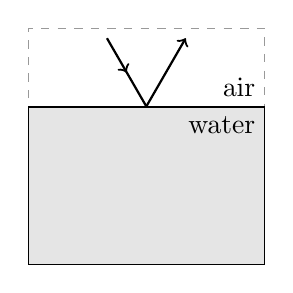
\begin{tikzpicture}
                \draw[dashed,white!60!black] (-1.5,-1) rectangle (1.5,2);
                %% water
                \node[draw,minimum width=3cm,minimum height=2cm,fill=white!90!black] (A) at (0,0) {};
                %% labels
                \node[anchor=north east] at (A.north east) {water};
                \node[anchor=south east] at (A.north east) {air};
                %% Ray
                \draw[thick,->] (A.north) -- ++(120:1) -- ++(300:0.5);
                \draw[thick,->] (A.north) -- ++(60:1);
            \end{tikzpicture}
        }
    \end{choices}
    \end{multicols}
\end{question}
}

\element{nysed}{
\begin{question}{Jan2004-Q31}
    A photon of light carries:
    \begin{choices}
      \correctchoice{both energy and momentum}
        \wrongchoice{energy, but not momentum}
        \wrongchoice{momentum, but not energy}
        \wrongchoice{neither momentum nor energy}
    \end{choices}
\end{question}
}


%% Section June2003
%%--------------------
\element{nysed}{
\begin{question}{June2003-Q26}
    In a vacuum, all electromagnetic waves have the same:
    \begin{multicols}{2}
    \begin{choices}
      \correctchoice{speed}
        \wrongchoice{wavelength}
        \wrongchoice{frequency}
        \wrongchoice{amplitude}
    \end{choices}
    \end{multicols}
\end{question}
}

\element{nysed}{
\begin{question}{June2003-Q27}
    The speed of light ($f=\SI{5.09e14}{\hertz}$) in a transparent material is \num{0.75} times its speed in air.
    The absolute index of refraction of the material is approximately:
    \begin{multicols}{4}
    \begin{choices}
      \correctchoice{\num{1.3}}
        \wrongchoice{\num{0.75}}
        \wrongchoice{\num{2.3}}
        \wrongchoice{\num{4.0}}
    \end{choices}
    \end{multicols}
\end{question}
}

\element{nysed}{
\begin{question}{June2003-Q28}
    Waves pass through a \SI{10}{\centi\meter} opening in a barrier without being diffracted.
    This observation provides evidence that the wavelength of the waves is:
    \begin{choices}
      \correctchoice{much shorter than \SI{10}{\centi\meter}}
        \wrongchoice{equal to \SI{10}{\centi\meter}}
        \wrongchoice{longer than \SI{10}{\centi\meter}, but shorter than \SI{20}{\centi\meter}}
        \wrongchoice{longer than \SI{10}{\centi\meter}}
    \end{choices}
\end{question}
}

\element{nysed}{
\begin{question}{June2003-Q32}
    Compared to a photon of red light, a photon of blue light has a:
    \begin{choices}
      \correctchoice{greater energy}
        \wrongchoice{longer wavelength}
        \wrongchoice{smaller momentum}
        \wrongchoice{lower frequency}
    \end{choices}
\end{question}
}

\element{nysed}{
\begin{question}{June2003-Q39}
    The diagram below represents a ray of monochromatic light ($f=\SI{5.09e14}{\hertz}$) passing from  medium $X$ ($n=\num{1.46}$) into fused quartz.
    %% fused quartz = 1.458
    \begin{center}
    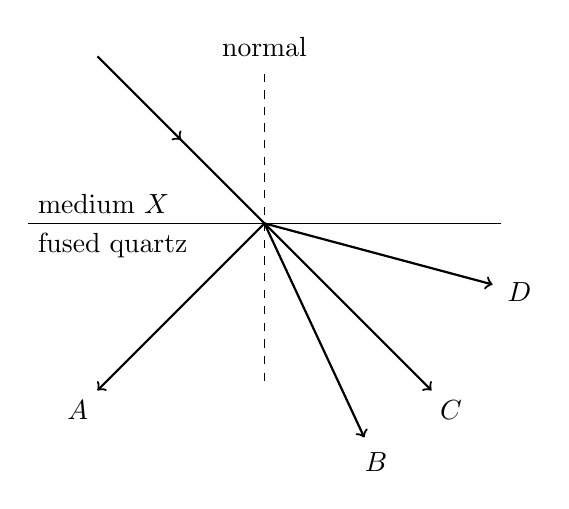
\begin{tikzpicture}
        %% axis
        \draw (-3,0) -- (3,0);
        \draw[dashed] (0,-2) -- (0,2) node[anchor=south] {normal};
        \node[anchor=south west] at (-3,0) {medium $X$};
        \node[anchor=north west] at (-3,0) {fused quartz};
        %% incident
        \draw[thick,->] (0,0) -- (135:3) --++(315:1.5);
        %% refracted
        \foreach \x/\y in {225/A,295/B,315/C,345/D}
            \draw[thick,->] (0,0) -- (\x:3) node[anchor=center,shift={(\x:1em)}] {$\y$};
    \end{tikzpicture}
    \end{center}
    Which path will the ray follow in the quartz?
    \begin{multicols}{4}
    \begin{choices}[o]
        \wrongchoice{$A$}
        \wrongchoice{$B$}
      \correctchoice{$C$}
        \wrongchoice{$D$}
    \end{choices}
    \end{multicols}
\end{question}
}


%% Section Jan2003
%%--------------------
\element{nysed}{
\begin{question}{Jan2003-Q30}
    In a certain material, a beam of monochromatic light ($f = \SI{5.09e14}{\hertz}$) has a speed of \SI{2.25e8}{\meter\per\second}.
    The material could be:
    \begin{multicols}{2}
    \begin{choices}
      \correctchoice{water}
        \wrongchoice{glycerol}
        \wrongchoice{flint glass}
        \wrongchoice{crown glass}
    \end{choices}
    \end{multicols}
\end{question}
}

\element{nysed}{
\begin{question}{Jan2003-Q31}
    Orange light has a frequency of \SI{5.0e14}{\hertz} in a vacuum.
    what is the wavelength of this light?
    \begin{multicols}{2}
    \begin{choices}
      \correctchoice{\SI{6e-7}{\meter}}
        \wrongchoice{\SI{2e-15}{\meter}}
        \wrongchoice{\SI{1.5e23}{\meter}}
        \wrongchoice{\SI{1.7e6}{\meter}}
    \end{choices}
    \end{multicols}
\end{question}
}

\element{nysed}{
\begin{question}{Jan2003-Q40}
    A photon of which electromagnetic radiation has the most energy?
    \begin{multicols}{2}
    \begin{choices}
      \correctchoice{x-ray}
        \wrongchoice{infrared}
        \wrongchoice{ultraviolet}
        \wrongchoice{microwave}
    \end{choices}
    \end{multicols}
\end{question}
}

\newcommand{\JanTwentyThreeQFortyEight}{
\begin{tikzpicture}
    %% NOTE: TODO: draw tikz
\end{tikzpicture}
}

\element{nysed}{
\begin{question}{Jan2003-Q48}
    The diagram below represents a light ray traveling from air to Lucite to medium Y and back into air.
    %% NOTE: lucite = 1.50
    \begin{center}
        \JanTwentyThreeQFortyEight
        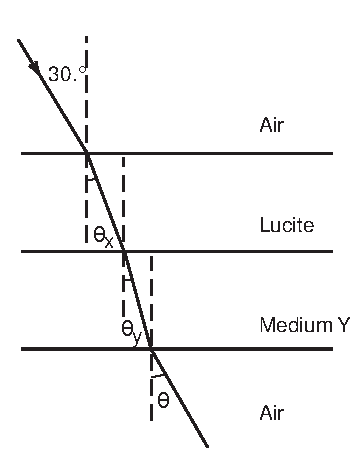
\includegraphics[keepaspectratio,scale=0.80]{Jan2003-Q48}
    \end{center}
    The sine of angle $\theta_x$ is:
    \begin{multicols}{2}
    \begin{choices}
      \correctchoice{\num{0.333}}
        \wrongchoice{\num{0.500}}
        \wrongchoice{\num{0.707}}
        \wrongchoice{\num{0.866}}
    \end{choices}
    \end{multicols}
\end{question}
}

\element{nysed}{
\begin{question}{Jan2003-Q49}
    The diagram below represents a light ray traveling from air to Lucite to medium $Y$ and back into air.
    \begin{center}
        \JanTwentyThreeQFortyEight
        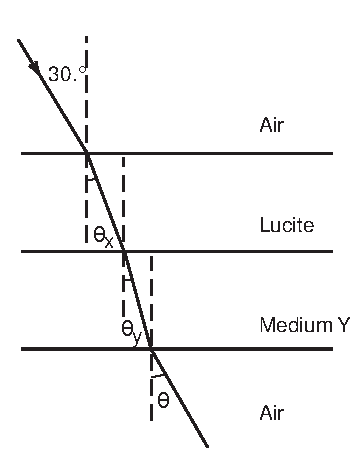
\includegraphics[keepaspectratio,scale=0.80]{Jan2003-Q48}
    \end{center}
    Light travels slowest in:
    \begin{choices}
      \correctchoice{medium $Y$, only}
        \wrongchoice{Lucite, only}
        \wrongchoice{air only}
        \wrongchoice{air, Lucite, and medium $Y$}
    \end{choices}
\end{question}
}


%% Section Aug2002
%%--------------------
\element{nysed}{
\begin{question}{Aug2002-Q32}
    A \SI{2.00e6}{\hertz} radio signal is sent a distance of \SI{7.30e10}{\meter} from Earth to a spaceship orbiting Mars.
    Approximately how much time does it take the radio signal to travel from Earth to the spaceship?
    \begin{multicols}{2}
    \begin{choices}
        \wrongchoice{\SI{4.11e-3}{\second}}
      \correctchoice{\SI{2.42e2}{\second}}
        \wrongchoice{\SI{2.19e8}{\second}}
        \wrongchoice{\SI{1.46e17}{\second}}
    \end{choices}
    \end{multicols}
\end{question}
}

\element{nysed}{
\begin{question}{Aug2002-Q33}
    A \SI{2.00e6}{\hertz} radio signal is sent a distance of \SI{7.30e10}{\meter} from Earth to a spaceship orbiting Mars.
    The spaceship is moving away from Earth when the radio signal is received.
    Compared to the frequency of the signal sent from Earth,
        the frequency of the signal received by the spaceship is:
    \begin{multicols}{3}
    \begin{choices}
      \correctchoice{lower}
        \wrongchoice{higher}
        \wrongchoice{the same}
    \end{choices}
    \end{multicols}
\end{question}
}

\element{nysed}{
\begin{question}{Aug2002-Q42}
    A monochromatic ray of light ($f=\SI{5.09e14}{\hertz}$) traveling in air is incident upon medium $A$ at an angle of \ang{45}.
    If the angle of refraction is \ang{29}, medium $A$ could be:
    \begin{multicols}{2}
    \begin{choices}
        \wrongchoice{water}
      \correctchoice{fused quartz}
        \wrongchoice{Lucite}
        \wrongchoice{flint glass}
    \end{choices}
    \end{multicols}
\end{question}
}


%% Section June2002
%%--------------------
\element{nysed}{
\begin{question}{June2002-Q19}
    In a vacuum, light with a frequency of \SI{5.0e14}{\hertz} has a wavelength of:
    \begin{multicols}{2}
    \begin{choices}
        \wrongchoice{\SI{6.0e-21}{\meter}}
      \correctchoice{\SI{6.0e-7}{\meter}}
        \wrongchoice{\SI{1.7e6}{\meter}}
        \wrongchoice{\SI{1.5e23}{\meter}}
    \end{choices}
    \end{multicols}
\end{question}
}

\element{nysed}{
\begin{question}{June2002-Q27}
    A beam of monochromatic light travels through flint glass,
        crown glass, Lucite, and water.
    The speed of the light beam is slowest in:
    %% flint glass 1.66
    %% crown glass 1.52
    %% Lucite      1.50
    %% Water       1.33
    \begin{multicols}{2}
    \begin{choices}
      \correctchoice{flint glass}
        \wrongchoice{crown glass}
        \wrongchoice{Lucite}
        \wrongchoice{water}
    \end{choices}
    \end{multicols}
\end{question}
}

\element{nysed}{
\begin{question}{June2002-Q31}
    Which characteristic of electromagnetic radiation is directly proportional to the energy of a photon?
    \begin{multicols}{2}
    \begin{choices}
        \wrongchoice{wavelength}
        \wrongchoice{period}
      \correctchoice{frequency}
        \wrongchoice{path}
    \end{choices}
    \end{multicols}
\end{question}
}

\element{nysed}{
\begin{question}{June2002-Q45}
    A beam of monochromatic light ($f=\SI{5.09e14}{\hertz}$) passes through parallel sections of glycerol,
        medium $X$, and medium $Y$ as shown in the diagram below.
    %% NOTE: glycerole 1.473
    \begin{center}
        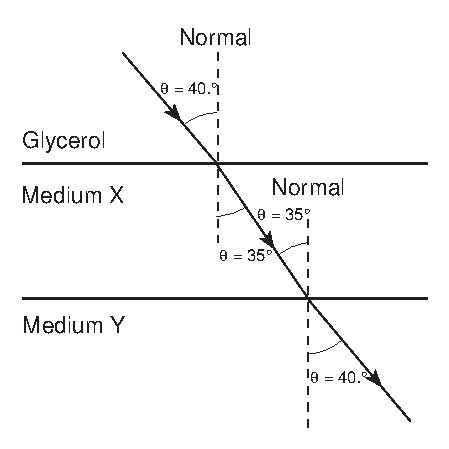
\includegraphics[keepaspectratio,scale=0.9]{June2002-Q45}
    \begin{tikzpicture}
        %% NOTE: TODO: draw tikz
    \end{tikzpicture}
    \end{center}
    What could be medium $X$ and medium $Y$ be?
    \begin{choices}
      \correctchoice{$X$ could be flint glass and $Y$ could be corn oil.}
        \wrongchoice{$X$ could be corn oil and $Y$ could be flint glass.}
        \wrongchoice{$X$ could be water and $Y$ could be glycerol.}
        \wrongchoice{$X$ could be glycerol and $Y$ could be water.}
    \end{choices}
\end{question}
}


%% Section Jan2002
%%--------------------
\element{nysed}{
\begin{question}{Jan2002-Q40}
    The diagram below shows a ray of light passing from medium $X$ into air.
    \begin{center}
    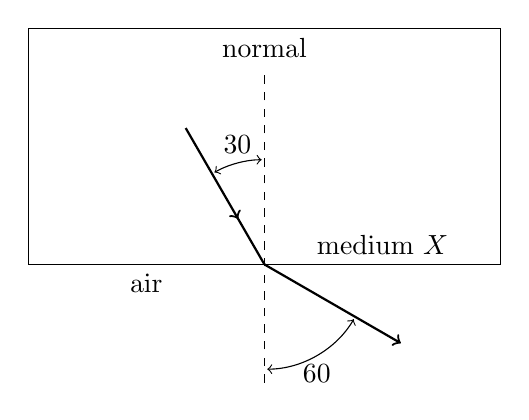
\begin{tikzpicture}
        %% Boundaries
        \draw (-3,0) rectangle (3,3);
        \node[anchor=south] at (1.5,0) {medium $X$};
        \node[anchor=north] at (-1.5,0) {air};
        %% normal
        \draw[dashed] (0,-1.5) -- (0,2.5) node[anchor=south] {normal};
        %% incident
        \draw[thick,->] (0,0) -- ++(120:2) --++(300:1.33);
        %% refracted
        \draw[<->,shorten <=1pt,shorten >=1pt] (0,1.33) arc (90:120:1.33) node[pos=0.5,anchor=south] {\ang{30}};
        \draw[thick,->] (0,0) -- ++(330:2);
        \draw[<->,shorten <=1pt,shorten >=1pt] (0,-1.33) arc (270:330:1.33) node[pos=0.5,anchor=north] {\ang{60}};
    \end{tikzpicture}
    \end{center}
    What is the absolute index of refraction of medium $X$?
    \begin{multicols}{2}
    \begin{choices}
        \wrongchoice{\num{0.500}}
        \wrongchoice{\num{2.00}}
      \correctchoice{\num{1.73}}
        \wrongchoice{\num{0.577}}
    \end{choices}
    \end{multicols}
\end{question}
}

\element{nysed}{
\begin{question}{Jan2002-Q42}
    What occurs when light passes from water into flint glass?
    \begin{choices}
      \correctchoice{Its speed decreases, its wavelength becomes shorter, and its frequency remains the same.}
        \wrongchoice{Its speed decreases, its wavelength becomes shorter, and its frequency increases.}
        \wrongchoice{Its speed increases, its wavelength becomes longer, and its frequency remains the same.}
        \wrongchoice{Its speed increases, its wavelength becomes longer, and its frequency decreases.}
    \end{choices}
\end{question}
}

\element{nysed}{
\begin{question}{Jan2002-Q44}
    The speed of light in a material is \SI{2.5e8}{\meter\per\second}.
    What is the absolute index of refraction of the material?
    \begin{multicols}{2}
    \begin{choices}
      \correctchoice{\num{1.20}}
        \wrongchoice{\num{2.50}}
        \wrongchoice{\num{7.50}}
        \wrongchoice{\num{0.833}}
    \end{choices}
    \end{multicols}
\end{question}
}

\element{nysed}{
\begin{question}{Jan2002-Q54}
    An astronomer on Earth studying light coming from a star notes that the observed light frequencies are lower than the actual emitted frequencies.
    The astronomer concludes that the distance between the star and Earth is:
    \begin{choices}
        \wrongchoice{decreasing}
      \correctchoice{increasing}
        \wrongchoice{unchanging}
    \end{choices}
\end{question}
}

\element{nysed}{
\begin{question}{Jan2002-Q55}
    compared to the wavelength of red light,
        the wavelength of yellow light is:
    \begin{multicols}{3}
    \begin{choices}
      \correctchoice{shorter}
        \wrongchoice{longer}
        \wrongchoice{the same}
    \end{choices}
    \end{multicols}
\end{question}
}

\element{nysed}{
\begin{question}{Jan2002-Q85}
    A helium-neon laser emits energy in the visible red region in the form of:
    \begin{multicols}{2}
    \begin{choices}
        \wrongchoice{alpha particles}
        \wrongchoice{gamma rays}
        \wrongchoice{electrons}
      \correctchoice{photons}
    \end{choices}
    \end{multicols}
\end{question}
}


%% Section June2001
%%--------------------
\element{nysed}{
\begin{question}{June2001-Q36}
    The diagram below shows light rays in air about to strike a glass window.
    \begin{center}
    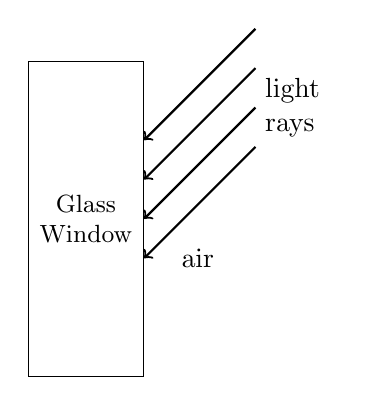
\begin{tikzpicture}
        %% labels
        \node[font=\small,draw,minimum width=1.33cm,minimum height=4cm,anchor=east,text centered,text width=3.5em] at (0,0) {Glass Window};
        \node[anchor=west] at (1em,-5mm) {air};
        %% light rays
        \foreach \y in {-5,0,5,10} \draw[thick,<-] (0,\y mm) -- ++(45:2);
        \node[anchor=west,text width=3em] at (45:2) {light rays};
    \end{tikzpicture}
    \end{center}
    When the rays reach the boundary between the air and the glass,
        the light is:
    \begin{choices}
        \wrongchoice{totally refracted}
        \wrongchoice{totally reflected}
        \wrongchoice{partially reflected and partially diffracted}
      \correctchoice{partially reflected and partially refracted}
    \end{choices}
\end{question}
}

\element{nysed}{
\begin{question}{June2001-Q40}
    A ray of monochromatic light traveling in air is incident on a plane mirror at an angle of \ang{30},
        as shown in the diagram below.
    \begin{center}
    \begin{tikzpicture}
        %% plane mirror
        \draw[pattern=north east lines] (0,-2) rectangle (0.2,2);
        \node[anchor=north west,text width=3em] at (0.2,2) {plane mirror};
        \node[anchor=north] at (-2,2) {air};
        %% normal
        \draw[dashed] (-4,0) -- (2,0) node[anchor=north east] {normal};
        %% incident
        \draw[thick,->] (0,0) -- (210:4) --++(30:2);
        \draw[<->,shorten <=1pt,shorten >=1pt] (-1.66,0) arc (180:210:1.66)
            node[pos=0.5,anchor=east] {\ang{30}};
    \end{tikzpicture}
    \end{center}
    The angle of reflection for the light ray is:
    \begin{multicols}{4}
    \begin{choices}
        \wrongchoice{\ang{15}}
      \correctchoice{\ang{30}}
        \wrongchoice{\ang{60}}
        \wrongchoice{\ang{90}}
    \end{choices}
    \end{multicols}
\end{question}
}

\element{nysed}{
\begin{question}{June2001-Q43}
    The diagram below represents monochromatic light incident on a pair of slits, $S_1$ and $S_2$,
        that are separated by a distance of \SI{2.0e-6}{\meter}.
    $A$, $B$, and $C$ are adjacent antinodal areas that appear on a screen \SI{1.0}{\meter} from the slits.
    The distance from $A$ to $B$ is \SI{0.34}{\meter}
    \begin{center}
        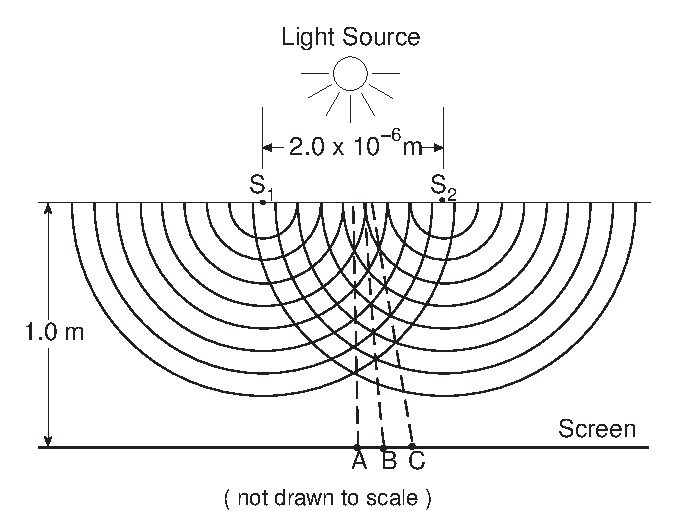
\includegraphics[keepaspectratio,scale=0.66]{June2001-Q43}
    \end{center}
    What is the wavelength of the incident light?
    \begin{multicols}{2}
    \begin{choices}
      \correctchoice{\SI{6.8e-7}{\meter}}
        \wrongchoice{\SI{5.9e-6}{\meter}}
        \wrongchoice{\SI{1.7e5}{\meter}}
        \wrongchoice{\SI{6.8e7}{\meter}}
    \end{choices}
    \end{multicols}
\end{question}
}

\element{nysed}{
\begin{question}{June2001-Q46}
    The diagram below shows a ray of light ($\lambda=\SI{5.9e-7}{\meter}$) traveling from air into medium $X$
    \begin{center}
    \begin{tikzpicture}
        %% axis
        \draw (-3,0) -- (3,0);
        \draw[dashed] (0,-3) -- (0,3) node[anchor=south] {normal};
        \node[anchor=south west] at (-3,0) {air};
        \node[anchor=north west] at (-3,0) {medium $X$};
        %% incident
        \draw[thick,->] (0,0) -- (120:3) -- ++(300:2);
        \draw[<->,shorten <=1pt,shorten >=1pt] (0,1.5) arc (90:120:1.5) node[pos=0.5,anchor=south] {\ang{30}};
        %% refracted
        \draw[thick,->] (0,0) -- (289:3);
        \draw[<->,shorten <=1pt,shorten >=1pt] (0,-2) arc (270:289:2) node[pos=0.5,anchor=north] {\ang{19}};
    \end{tikzpicture}
    \end{center}
    If the angle of incidence is \ang{30} and the angle of refraction is \ang{19}, medium $X$ could be:
    \begin{multicols}{2}
    \begin{choices}
        \wrongchoice{air}
        \wrongchoice{alcohol}
        %% Also: Canada turpentine or balsam of fir
      \correctchoice{Canada balsam}
        \wrongchoice{glycerol}
    \end{choices}
    \end{multicols}
\end{question}
}

\element{nysed}{
\begin{question}{June2001-Q47}
    As a monochromatic beam of light passes obliquely from flint glass into water,
        how do the characteristics of the beam of light change?
    \begin{choices}
        \wrongchoice{Its wavelength decreases and its frequency decreases}
        \wrongchoice{Its wavelength decreases and its frequency increases}
        \wrongchoice{Its wavelength increases and it bends toward the normal}
      \correctchoice{Its wavelength increases and it bends away from the normal}
    \end{choices}
\end{question}
}


%% Section Jan2001
%%--------------------
\element{nysed}{
\begin{question}{Jan2001-Q42}
    A beam of green light may have a frequency of:
    \begin{multicols}{2}
    \begin{choices}
        \wrongchoice{\SI{5.0e-7}{\hertz}}
        \wrongchoice{\SI{1.5e2}{\hertz}}
        \wrongchoice{\SI{3.0e8}{\hertz}}
      \correctchoice{\SI{6.0e14}{\hertz}}
    \end{choices}
    \end{multicols}
\end{question}
}

\element{nysed}{
\begin{question}{Jan2001-Q46}
    When yellow light having a wavelength of \SI{5.8e-7}{\meter} shines through two slits \SI{2.0e-4}{\meter} apart,
        an interference patter is formed on a screen \SI{2.0}{\meter} from the slits.
    What distance separates the first-order maximum and the central maximum?
    \begin{multicols}{2}
    \begin{choices}
        \wrongchoice{\SI{5.8e-11}{\meter}}
        \wrongchoice{\SI{1.5e-3}{\meter}}
      \correctchoice{\SI{5.8e-3}{\meter}}
        \wrongchoice{\SI{6.9e2}{\meter}}
    \end{choices}
    \end{multicols}
\end{question}
}

\element{nysed}{
\begin{question}{Jan2001-Q47}
    The diagram below shows parallel rays of light incident on an irregular surface.
    \begin{center}
        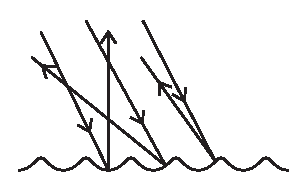
\includegraphics[keepaspectratio,scale=0.9]{Jan2001-Q47}
    \end{center}
    Which phenomenon of light is illustrated by the diagram?
    \begin{multicols}{2}
    \begin{choices}
        \wrongchoice{diffraction}
        \wrongchoice{refraction}
        \wrongchoice{regular reflection}
      \correctchoice{diffuse reflection}
    \end{choices}
    \end{multicols}
\end{question}
}

\element{nysed}{
\begin{question}{Jan2001-Q48}
    What is the speed of light in a medium having an absolute index of refraction of \num{2.3}?
    \begin{multicols}{2}
    \begin{choices}
        \wrongchoice{\SI{0.77e8}{\meter\per\second}}
      \correctchoice{\SI{1.3e8}{\meter\per\second}}
        \wrongchoice{\SI{1.5e8}{\meter\per\second}}
        \wrongchoice{\SI{2.3e8}{\meter\per\second}}
    \end{choices}
    \end{multicols}
\end{question}
}

\element{nysed}{
\begin{question}{Jan2001-Q50}
    Compared to wavelengths of visible light,
        the wavelength of ultraviolet light are:
    \begin{multicols}{3}
    \begin{choices}
      \correctchoice{shorter}
        \wrongchoice{longer}
        \wrongchoice{the same}
    \end{choices}
    \end{multicols}
\end{question}
}

\element{nysed}{
\begin{question}{Jan2001-Q52}
    The diagram below shows a ray of light passing through two media.
    \begin{center}
    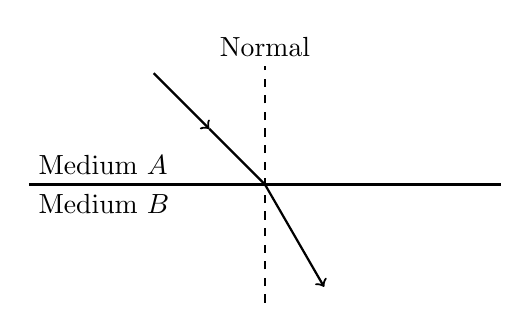
\begin{tikzpicture}
        %% Incident
        \draw[thick,->] (135:2) -- (135:1.00);
        \draw[thick] (135:1.00) -- (135:0);
        %% Refracted
        \draw[thick,->] (0,0) -- (-60:1.5);
        %% Normal
        \draw[thick,dashed] (0,-1.5) -- (0,1.5)
            node[pos=1.0,anchor=south] {Normal};
        %% Glass and Air
        \draw[thick] (-3,0) -- (3,0);
        \node[anchor=south west] at (-3,0) {Medium $A$};
        \node[anchor=north west] at (-3,0) {Medium $B$};
    \end{tikzpicture}
    \end{center}
    When the wave travels from medium $A$ into medium $B$,
        its speed:
    \begin{choices}
      \correctchoice{decreases}
        \wrongchoice{increases}
        \wrongchoice{remains the same}
    \end{choices}
\end{question}
}

\element{nysed}{
\begin{question}{Jan2001-Q53}
    Experiments performed with light indicate that light exhibits:
    \begin{choices}
        \wrongchoice{particle properties, only}
        \wrongchoice{wave properties, only}
      \correctchoice{both particle and wave properties}
        \wrongchoice{neither particle nor wave properties}
    \end{choices}
\end{question}
}

\element{nysed}{
\begin{question}{Jan2001-Q54}
    What is the energy of a quantum of light having a frequency of \SI{6.0e14}{\hertz}?
    \begin{multicols}{2}
    \begin{choices}
        \wrongchoice{\SI{1.6e-19}{\joule}}
      \correctchoice{\SI{4.0e-19}{\joule}}
        \wrongchoice{\SI{3.0e8}{\joule}}
        \wrongchoice{\SI{5.0e-7}{\joule}}
    \end{choices}
    \end{multicols}
\end{question}
}


%% Section June2000
%%--------------------
\element{nysed}{
\begin{question}{June2000-Q41}
    A monochromatic beam of light has a frequency of \SI{6.5e14}{\hertz}.
    What color is the light?
    %% let f = 6.5e14 Hz
    %% then \lambda = 460 nm
    \begin{multicols}{2}
    \begin{choices}
        \wrongchoice{yellow}
        \wrongchoice{orange}
      \correctchoice{violet}
        \wrongchoice{blue}
    \end{choices}
    \end{multicols}
\end{question}
}

\element{nysed}{
\begin{question}{June2000-Q42}
    Two waves having the same amplitude and the same frequency pass simultaneously through a uniform medium.
    Maximum destructive interference occurs when the phase difference between the two waves is:
    \begin{multicols}{4}
    \begin{choices}
        \wrongchoice{\ang{0}}
        \wrongchoice{\ang{90}}
      \correctchoice{\ang{180}}
        \wrongchoice{\ang{360}}
    \end{choices}
    \end{multicols}
\end{question}
}

\newcommand{\JuneTwoThousandQFortyFive}{
    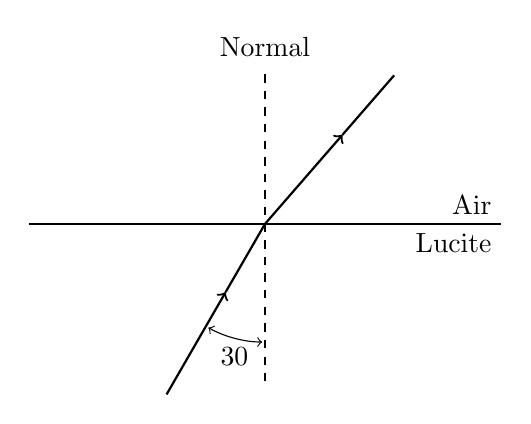
\begin{tikzpicture}
        %% Incident
        \draw[thick,->] (240:2.5) -- (240:1);
        \draw[thick] (240:1) -- (240:0);
        \draw[<->,shorten <=1pt,shorten >=1pt] (270:1.5) arc (270:240:1.5)
            node[pos=0.5,anchor=north] {\ang{30}};
        %% Refracted
        \draw[thick,->] (49:0) -- (49:1.5);
        \draw[thick] (49:1.5) -- (49:2.5);
        %% Normal
        \draw[thick,dashed] (0,-2.0) -- (0,2.0)
            node[pos=1.0,anchor=south] {Normal};
        %% Air and Lucite n = 1.5
        \draw[thick] (-3,0) -- (3,0);
        \node[anchor=south east] at (3,0) {Air};
        \node[anchor=north east] at (3,0) {Lucite};
    \end{tikzpicture}
}

\element{nysed}{
\begin{question}{June2000-Q45}
    The diagram below which represents a beam of monochromatic light ($\lambda=\SI{5.9e-7}{\meter}$) traveling from Lucite into air.
    \begin{center}
        \JuneTwoThousandQFortyFive
    \end{center}
    What is the measure of the angle of refraction?
    [Use a protractor or a mathematical calculation.]
    \begin{multicols}{4}
    \begin{choices}
        \wrongchoice{\ang{19}}
        \wrongchoice{\ang{30}}
      \correctchoice{\ang{49}}
        \wrongchoice{\ang{60}}
    \end{choices}
    \end{multicols}
\end{question}
}

\element{nysed}{
\begin{question}{June2000-Q46}
    The diagram below which represents a beam of monochromatic light ($\lambda=\SI{5.9e-7}{\meter}$) traveling from Lucite into air.
    \begin{center}
        \JuneTwoThousandQFortyFive
    \end{center}
    The speed of the light in Lucite is:
    \begin{multicols}{2}
    \begin{choices}
        \wrongchoice{\SI{1.5e8}{\meter\per\second}}
      \correctchoice{\SI{2.0e8}{\meter\per\second}}
        \wrongchoice{\SI{3.0e8}{\meter\per\second}}
        \wrongchoice{\SI{4.5e8}{\meter\per\second}}
    \end{choices}
    \end{multicols}
\end{question}
}

\element{nysed}{
\begin{question}{June2000-Q47}
    The diagram below which represents a beam of monochromatic light ($\lambda=\SI{5.9e-7}{\meter}$) traveling from Lucite into air
    \begin{center}
        \JuneTwoThousandQFortyFive
    \end{center}
    The critical angle for the Lucite-air boundary is approximately:
    \begin{multicols}{4}
    \begin{choices}
        \wrongchoice{\ang{67}}
      \correctchoice{\ang{42}}
        \wrongchoice{\ang{48}}
        \wrongchoice{\ang{33}}
    \end{choices}
    \end{multicols}
\end{question}
}

\element{nysed}{
\begin{question}{June2000-Q48}
    A light ray is incident on a plane mirror as shown in the diagram below.
    \begin{center}
    \begin{tikzpicture}
        %% plane mirror
        \draw (-3,0) -- (3,0);
        \node[pattern=north east lines,anchor=north,minimum width=6cm] at (0,0) {};
        \node[anchor=north east] at (3,-1em) {plane mirror};
        %% incident
        \draw[thick,-latex] (0,0) -- (135:4) --++(315:2)
            node[pos=1.0,anchor=south east,rotate=-45] {incident ray};
        %% reflected
        \foreach \x/\y in {90/A,65/B,45/C,25/D} 
            \draw[thick,-latex] (0,0) -- (\x:3) node[anchor=center,shift={(\x:1em)}] {$\y$};
    \end{tikzpicture}
    \end{center}
    Which ray best represents the reflected ray?
    \begin{multicols}{4}
    \begin{choices}[o]
        \wrongchoice{$A$}
        \wrongchoice{$B$}
      \correctchoice{$C$}
        \wrongchoice{$D$}
    \end{choices}
    \end{multicols}
\end{question}
}

\element{nysed}{
\begin{question}{June2000-Q49}
    What occurs as a ray of light passes from air into water?
    \begin{choices}
      \correctchoice{The ray must decrease in speed}
        \wrongchoice{The ray must increase in speed}
        \wrongchoice{The ray must decrease in frequency}
        \wrongchoice{The ray must increase in frequency}
    \end{choices}
\end{question}
}

\element{nysed}{
\begin{question}{June2000-Q51}
    In which part of the electromagnetic spectrum does a photon have the greatest energy?
    \begin{multicols}{2}
    \begin{choices}
        \wrongchoice{red}
        \wrongchoice{infrared}
        \wrongchoice{violet}
      \correctchoice{ultraviolet}
    \end{choices}
    \end{multicols}
\end{question}
}

\element{nysed}{
\begin{question}{June2000-Q52}
    If all parts of a light beam have a constant phase relationship,
        with the same wavelength and frequency,
        the light beam is:
    \begin{choices}
      \correctchoice{monochromatic and coherent}
        \wrongchoice{monochromatic and incoherent}
        \wrongchoice{polychromatic and coherent}
        \wrongchoice{polychromatic and incoherent}
    \end{choices}
\end{question}
}


%% Section June1999
%%--------------------

%% NOTE: Q45 requires graphics

\element{nysed}{
\begin{question}{June1999-Q47}
    When a student looks into a plane mirror,
        she sees a virtual image of herself.
    However, when she looks into a sheet of paper,
        no such image forms.
    Which light phenomenon occurs at the surface of the paper?
    \begin{multicols}{2}
    \begin{choices}
        \wrongchoice{regular reflection}
      \correctchoice{diffuse reflection}
        \wrongchoice{polarization}
        \wrongchoice{resonance}
    \end{choices}
    \end{multicols}
\end{question}
}

\element{nysed}{
\begin{question}{June1999-Q48}
    Light from the star Betelgeuse displays a Doppler red shift.
    This shift is best explained by assuming that Betelgeuse is:
    \begin{choices}
        \wrongchoice{decreasing in temperature}
        \wrongchoice{increasing in temperature}
        \wrongchoice{moving toward Earth}
      \correctchoice{moving away from Earth}
    \end{choices}
\end{question}
}

\element{nysed}{
\begin{question}{June1999-Q49}
    Light with a wavelength of \SI{6.0e-7}{\meter} passes through a pair of narrow slits and falls on a screen \SI{2.0}{\meter} away.
    If the distance between two adjacent bright bands on the screen is \SI{3.0e-2}{\meter},
        what is the distance between the slits?
    \begin{multicols}{2}
    \begin{choices}
        \wrongchoice{\SI{9.0e-9}{\meter}}
        \wrongchoice{\SI{1.0e-5}{\meter}}
      \correctchoice{\SI{4.0e-5}{\meter}}
        \wrongchoice{\SI{2.5e4}{\meter}}
    \end{choices}
    \end{multicols}
\end{question}
}

%% NOTE: The graphics are possible duplicates
%% NOTE: June1999-Q52 to June1999-Q57 are missing

\element{nysed}{
\begin{question}{June1999-Q51}
    Which diagram best represents the path of light rays passing through a glass prism?
    \begin{multicols}{2}
    \begin{choices}
        \wrongchoice{
            \begin{tikzpicture}
                %% NOTE: TODO: finish this
            \end{tikzpicture}
        }
    \end{choices}
    \end{multicols}
\end{question}
}


%% Section June1998
%%--------------------
\element{nysed}{
\begin{question}{June1998-Q43}
    A ray of light strikes a plane mirror at an angle of incidence equal to \ang{35}.
    The angle between the incident ray and the reflected ray is:
    \begin{multicols}{4}
    \begin{choices}
        \wrongchoice{\ang{0}}
        \wrongchoice{\ang{35}}
        \wrongchoice{\ang{55}}
      \correctchoice{\ang{70}}
    \end{choices}
    \end{multicols}
\end{question}
}

\element{nysed}{
\begin{question}{June1998-Q44}
    A ray of light ($\lambda = \SI{5.9e-7}{\meter}$) traveling in air is incident on an interface with medium $X$ at an angle of \ang{30}.
    The angle of refraction for the light ray in medium $X$ is \ang{12}.
    Medium $X$ could be:
    \begin{multicols}{2}
    \begin{choices}
        \wrongchoice{alcohol}
        \wrongchoice{corn oil}
      \correctchoice{diamond}
        \wrongchoice{flint glass}
    \end{choices}
    \end{multicols}
\end{question}
}

%% NOTE: June1998-Q46 requires graphic
%% NOTE: June1998-Q48 requires graphic

\element{nysed}{
\begin{question}{June1998-Q52}
    A ray of monochromatic light is traveling in flint glass.
    The ray strikes the flint glass--air interface at an angle of incident greater than the critcal angle for fling glass.
    Which diagram best represents the path of this light ray?
    %% flint glass = 1.66
    \begin{multicols}{2}
    \begin{choices}
        \AMCboxDimensions{down=-1.2cm}
        \correctchoice{
            \begin{tikzpicture}[scale=0.75]
                %% axis
                \draw (-2,0) -- (2,0);
                \draw[dashed] (0,-2) -- (0,2) node[anchor=south] {normal};
                \node[anchor=south east,text width=3em,align=right] at (+2,0) {flint glass};
                \node[anchor=north west] at (-2,0) {air};
                %% incident
                \draw[thick,->] (135:2) -- (135:1);
                \draw[thick] (135:1) -- (135:0);
                %% reflected/refracted
                \draw[thick,->] (45:0) -- (45:1);
                \draw[thick] (45:1) -- (45:2);
            \end{tikzpicture}
        }
        \wrongchoice{
            \begin{tikzpicture}[scale=0.75]
                %% axis
                \draw (-2,0) -- (2,0);
                \draw[dashed] (0,-2) -- (0,2) node[anchor=south] {normal};
                \node[anchor=south east,text width=3em,align=right] at (+2,0) {flint glass};
                \node[anchor=north west] at (-2,0) {air};
                %% incident
                \draw[thick,->] (135:2) -- (135:1);
                \draw[thick] (135:1) -- (135:0);
                %% reflected/refracted
                \draw[thick,->] (315:0) -- (315:1);
                \draw[thick] (315:1) -- (315:2);
            \end{tikzpicture}
        }
        \wrongchoice{
            \begin{tikzpicture}[scale=0.75]
                %% axis
                \draw (-2,0) -- (2,0);
                \draw[dashed] (0,-2) -- (0,2) node[anchor=south] {normal};
                \node[anchor=south east,text width=3em,align=right] at (+2,0) {flint glass};
                \node[anchor=north west] at (-2,0) {air};
                %% incident
                \draw[thick,->] (135:2) -- (135:1);
                \draw[thick] (135:1) -- (135:0);
                %% reflected/refracted
                \draw[thick,->] (335:0) -- (335:1);
                \draw[thick] (335:1) -- (335:2);
            \end{tikzpicture}
        }
        \wrongchoice{
            \begin{tikzpicture}[scale=0.75]
                %% axis
                \draw (-2,0) -- (2,0);
                \draw[dashed] (0,-2) -- (0,2) node[anchor=south] {normal};
                \node[anchor=south east,text width=3em,align=right] at (+2,0) {flint glass};
                \node[anchor=north west] at (-2,0) {air};
                %% incident
                \draw[thick,->] (135:2) -- (135:1);
                \draw[thick] (135:1) -- (135:0);
                %% no reflected/refracted
            \end{tikzpicture}
        }
    \end{choices}
    \end{multicols}
\end{question}
}


%% Section June1997
%%--------------------
\element{nysed}{
\begin{question}{June1997-Q37}
    The frequency of a light wave is \SI{5.0e15}{\hertz}.
    What is the period of the wave?
    \begin{multicols}{2}
    \begin{choices}
        \wrongchoice{\SI{1.7e6}{\second}}
      \correctchoice{\SI{2.0e-15}{\second}}
        \wrongchoice{\SI{6.0e-7}{\second}}
        \wrongchoice{\SI{5.0e-14}{\second}}
    \end{choices}
    \end{multicols}
\end{question}
}

\element{nysed}{
\begin{question}{June1997-Q38}
    The amplitude of a sound wave is to its loudness as the amplitude of a light wave is to its:
    \begin{multicols}{2}
    \begin{choices}
      \correctchoice{brightness}
        \wrongchoice{frequency}
        \wrongchoice{color}
        \wrongchoice{speed}
    \end{choices}
    \end{multicols}
\end{question}
}

%% NOTE: alternate question
\element{nysed}{
\begin{question}{June1997-Q38A}
    The frequency of a sound wave is to its pitch as the frequency of a light wave is to its:
    \begin{multicols}{2}
    \begin{choices}
        \wrongchoice{brightness}
        \wrongchoice{frequency}
      \correctchoice{color}
        \wrongchoice{speed}
    \end{choices}
    \end{multicols}
\end{question}
}

\element{nysed}{
\begin{question}{June1997-Q39}
    The speed of light in glycerol is approximately:
    \begin{multicols}{2}
    \begin{choices}
        \wrongchoice{\SI{1.0e7}{\meter\per\second}}
      \correctchoice{\SI{2.0e8}{\meter\per\second}}
        \wrongchoice{\SI{3.0e8}{\meter\per\second}}
        \wrongchoice{\SI{4.4e8}{\meter\per\second}}
    \end{choices}
    \end{multicols}
\end{question}
}

\element{nysed}{
\begin{question}{June1997-Q42}
    The diagram below shows a ray of monochromatic light incident on an alcohol-flint glass interface.
    \begin{center}
    \begin{tikzpicture}
        \draw (-3,0) -- (3,0);
        \draw[dashed] (0,-1) -- (0,2) node[anchor=south] {Normal};
        \draw[very thick,->] (0,0) -- (135:3) -- ++(315:1.5);
        \node[anchor=south east] at (3,0) {Alcohol};
        \node[anchor=north east] at (3,0) {Flint Glass};
    \end{tikzpicture}
    \end{center}
    What occurs as the light travels from alcohol into flint glass?
    \begin{choices}
      \correctchoice{The speed of the light decreases and the ray bends toward the normal.}
        \wrongchoice{The speed of the light decreases and the ray bends away from the normal.}
        \wrongchoice{The speed of the light increases and the ray bends toward the normal.}
        \wrongchoice{The speed of the light increases and the ray bends away from the normal.}
    \end{choices}
\end{question}
}

\element{nysed}{
\begin{question}{June1997-Q44}
    The absolute index of refraction for a substance is \num{2.0} for light having a wavelength of \SI{5.9e-7}{\meter}.
    In this substance,
        what is the critical angle for light incident on a boundary with air?
    \begin{multicols}{4}
    \begin{choices}
      \correctchoice{\ang{30}}
        \wrongchoice{\ang{45}}
        \wrongchoice{\ang{60}}
        \wrongchoice{\ang{90}}
    \end{choices}
    \end{multicols}
\end{question}
}

\element{nysed}{
\begin{question}{June1997-Q45}
    A ray of monochromatic light ($\lambda=\SI{5.9e-7}{\meter}$) traveling in air is incident on an interface with a liquid at an angle of \ang{45},
        as shown in the diagram below.
    \begin{center}
    \begin{tikzpicture}
        \draw (-3,0) -- (3,0);
        \draw[dashed] (0,-1) -- (0,3) node[anchor=south] {Normal};
        \draw[very thick,->] (0,0) -- (135:4) -- ++(315:2);
        \draw[<->,shorten <=1pt,shorten >=1pt] (90:1.33) arc (90:135:1.33)
            node[pos=0.5,anchor=south] {\ang{45}};
        \node[anchor=south east] at (3,0) {Air $n=1.0$};
        \node[anchor=north east] at (3,0) {Liquid $n=1.4$};
    \end{tikzpicture}
    \end{center}
    If the absolute index of refraction of the liquid is \num{1.4},
        the angle of refraction for the light ray is closest to:
    \begin{multicols}{4}
    \begin{choices}
        \wrongchoice{\ang{10}}
        \wrongchoice{\ang{20}}
      \correctchoice{\ang{30}}
        \wrongchoice{\ang{40}}
    \end{choices}
    \end{multicols}
\end{question}
}

\element{nysed}{
\begin{question}{June1997-Q46}
    Which phenomenon can occur with light, but \emph{not} with sound?
    \begin{multicols}{2}
    \begin{choices}
        \wrongchoice{interference}
      \correctchoice{polarization}
        \wrongchoice{refraction}
        \wrongchoice{the Doppler effect}
    \end{choices}
    \end{multicols}
\end{question}
}

%% NOTE: questionmult with varying amplitude
\element{nysed}{
\begin{question}{June1997-Q48}
    Which diagram best represents light emitted from a coherent light source?
    %% coherent = same frequency and phase
    \begin{multicols}{2}
    \begin{choices}
        \AMCboxDimensions{down=-0.4cm}
        \wrongchoice{
            \begin{tikzpicture}[x=0.07\linewidth]
                \draw[dashed,white!60!black] (0,0.5) rectangle (12.6,2);
                %% change frequency
                \foreach \a in {1.0,1.2,1.4}
                    \draw[domain=0:4*pi,smooth,line width=1pt] plot (\x, {\a - 0.25*cos(\a*\x r)});
            \end{tikzpicture}
        }
        \wrongchoice{
            \begin{tikzpicture}[x=0.07\linewidth]
                \draw[dashed,white!60!black] (0,0.5) rectangle (12.6,2);
                %% change phase
                \foreach \a in {1.0,1.2,1.4}
                    \draw[domain=0:4*pi,smooth,line width=1pt] plot (\x, {\a - 0.25*cos(deg(\x+2*\a))});
            \end{tikzpicture}
        }
        \wrongchoice{
            \begin{tikzpicture}[x=0.07\linewidth]
                \draw[dashed,white!60!black] (0,0.5) rectangle (12.6,2);
                %% change amplitude and frequency
                \foreach \a in {1.0,1.2,1.4}
                    \draw[domain=0:4*pi,smooth,line width=1pt] plot (\x, {\a - \a*0.2*cos(deg(\a*\x))});
            \end{tikzpicture}
        }
        \correctchoice{
            \begin{tikzpicture}[x=0.07\linewidth]
                \draw[dashed,white!60!black] (0,0.5) rectangle (12.6,2);
                %% change nothing
                \foreach \a in {1.0,1.2,1.4}
                    \draw[domain=0:4*pi,smooth,line width=1pt] plot (\x, {\a - 0.25*cos(deg(\x))});
            \end{tikzpicture}
        }
    \end{choices}
    \end{multicols}
\end{question}
}


%% Section June1996
%%--------------------
\element{nysed}{
\begin{question}{June1996-Q35}
    Electromagnetic waves can be generated by accelerating:
    \begin{multicols}{2}
    \begin{choices}
        \wrongchoice{a hydrogen atom}
        \wrongchoice{a photon}
        \wrongchoice{a neutron}
      \correctchoice{an electron}
    \end{choices}
    \end{multicols}
\end{question}
}

\element{nysed}{
\begin{question}{June1996-Q41}
    A beam of monochromatic light ($\lambda = \SI{5.9e-7}{\meter}$) crosses a boundary from air into Lucite at an angle of incidence of \ang{45}.
    The angle of refraction is approximately:
    \begin{multicols}{4}
    \begin{choices}
        \wrongchoice{\ang{63}}
        \wrongchoice{\ang{56}}
        \wrongchoice{\ang{37}}
      \correctchoice{\ang{28}}
    \end{choices}
    \end{multicols}
\end{question}
}

\element{nysed}{
\begin{question}{June1996-Q43}
    The speed of light in a material is \SI{2.5e8}{\meter\per\second}.
    What is the absolute index of refraction of the material?
    \begin{multicols}{4}
    \begin{choices}
      \correctchoice{1.2}
        \wrongchoice{2.5}
        \wrongchoice{7.5}
        \wrongchoice{0.83}
    \end{choices}
    \end{multicols}
\end{question}
}

\element{nysed}{
\begin{question}{June1996-Q45}
    A laser beam does \emph{not} disperse as it passes through a prism because the laser beam is:
    \begin{multicols}{2}
    \begin{choices}
      \correctchoice{monochromatic}
        \wrongchoice{polychromatic}
        \wrongchoice{polarized}
        \wrongchoice{longitudinal}
    \end{choices}
    \end{multicols}
\end{question}
}

\element{nysed}{
\begin{question}{June1996-Q47}
    In the diagram below, monochromatic light ($\lambda=\SI{5.9e-2}{\meter}$)
        in the air is about to travel through crown glass, water and diamond.
    \begin{center}
    \begin{tikzpicture}
        \begin{scope}[xshift=-1.5cm,yshift=2mm]
            \node[anchor=south] at (0,1.5) {$\lambda=\SI{5.9e-7}{\meter}$};
            \node[anchor=north] at (0,0) {air};
            \foreach \y in {2,6,10,14} \draw[thick,->] (-1,\y mm) -- (1,\y mm);
        \end{scope}
        \begin{scope}[xshift=+1.5cm]
            \draw (-0.9,1.8) -- (0.9,1.8);
            \draw[thick,fill=white] (-1,2) -- (-0.8,0) -- (0.8,0) -- (1,2) -- (0.9,2) -- (0.7,0.1) -- (-0.7,0.1) -- (-0.9,2) -- cycle;
            \node[pin={[pin edge={latex-}]15:crown glass}] at (0.9,1.8) {};
            \node[pin={[black,pin edge={latex-},pin distance=1cm]15:water}] at (0.2,1) {};
            \node[anchor=south,diamond,draw] at (0,0.1) {};
            \node[pin={[black,pin edge={latex-},pin distance=1cm]15:diamond}] at (0.2,0.3) {};
        \end{scope}
    \end{tikzpicture}
    \end{center}
    In which substance does the light travel the slowest?
    \begin{multicols}{2}
    \begin{choices}
        \wrongchoice{air}
      \correctchoice{diamond}
        \wrongchoice{water}
        \wrongchoice{crown glass}
    \end{choices}
    \end{multicols}
\end{question}
}

%\element{nysed}{
%\begin{question}{June1996-Q50}
%    The diagram below shows sunglasses being used to eliminate glare.
%    \begin{center}
%        %% NOTE: needs picture
%    \end{center}
%    Which phenomenon of light is represented in the diagram?
%    \begin{multicols}{2}
%    \begin{choices}
%        \wrongchoice{dispersion}
%        \wrongchoice{diffraction}
%        \wrongchoice{internal reflection}
%        \wrongchoice{polarization}
%    \end{choices}
%    \end{multicols}
%\end{question}
%}

\element{nysed}{
\begin{question}{June1996-Q54}
    Light ($\lambda=\SI{5.9e-7}{\meter}$) travels through a solution.
    If the absolute index of refraction of the solution is increased,
        the critical angle will:
    \begin{choices}
      \correctchoice{decrease}
        \wrongchoice{increase}
        \wrongchoice{remain the same}
    \end{choices}
\end{question}
}

\element{nysed}{
\begin{question}{June1996-Q55}
    An astronomer on Earth studying light coming from a star notes that the observed light frequencies are lower than the actual emitted frequencies.
    The astronomer concludes that the distance between the star and Earth is:
    \begin{choices}
        \wrongchoice{decreasing}
      \correctchoice{increasing}
        \wrongchoice{not changing}
    \end{choices}
\end{question}
}


%% Section June1995
%%--------------------
\element{nysed}{
\begin{question}{June1995-Q33}
    In a nondispersive medium,
        the speed of a light wave depends on:
    \begin{choices}
        \wrongchoice{its wavelength}
        \wrongchoice{its amplitude}
        \wrongchoice{its frequency}
      \correctchoice{the nature of the medium}
    \end{choices}
\end{question}
}

\element{nysed}{
\begin{question}{June1995-Q43}
    In a vacuum, a monochromatic beam of light has a frequency of \SI{6.3e14}{\hertz}.
    What color is the light?
    \begin{multicols}{2}
    \begin{choices}
        \wrongchoice{red}
        \wrongchoice{yellow}
        \wrongchoice{green}
      \correctchoice{blue}
    \end{choices}
    \end{multicols}
\end{question}
}

\element{nysed}{
\begin{question}{June1995-Q45}
    A beam of light crosses a boundary between two different media.
    Refraction can occur if:
    \begin{choices}
        \wrongchoice{the angle of incidence is \ang{0}}
        \wrongchoice{there is no change in the speed of the wave}
      \correctchoice{the media have different indices of refraction}
        \wrongchoice{all of the light is reflected}
    \end{choices}
\end{question}
}

\element{nysed}{
\begin{question}{June1995-Q46}
    What is the energy of a photon with a frequency of \SI{5.0e14}{\hertz}?
    \begin{multicols}{2}
    \begin{choices}
        \wrongchoice{\SI{3.3}{\eV}}
        \wrongchoice{\SI{3.2e-6}{\eV}}
        \wrongchoice{\SI{3.0e48}{\joule}}
      \correctchoice{\SI{3.0e-19}{\joule}}
    \end{choices}
    \end{multicols}
\end{question}
}

\element{nysed}{
\begin{question}{June1995-Q47}
    The diagram below shows white light being dispersed as it passes from air into a glass prism.
    \begin{center}
    \begin{tikzpicture}
        %% prism
        \draw (-2,0) -- (0,3.46) -- (2,0) -- cycle;
        \node[anchor=south] at (0,0) {glass};
        %% white light
        \draw[thick,-latex] (-2,0) ++ (60:2) -- ++(190:3) --++(10:2);
        \path (-2,0) ++ (60:2) ++(190:3) node[anchor=south west,rotate=10] {white light};
        %% red and violet
        \draw[thick,-latex] (-2,0) ++ (60:2) -- ++(0:1.5) node[pos=0.5,anchor=south] {red};
        \draw[thick,-latex] (-2,0) ++ (60:2) -- ++(340:1.5) node[pos=0.5,anchor=north,rotate=-20] {violet};
    \end{tikzpicture}
    \end{center}
    This phenomenon occurs because, in glass, each frequency of light has a different:
    \begin{choices}
        \wrongchoice{intensity}
        \wrongchoice{amplitude}
        \wrongchoice{angle of incidence}
      \correctchoice{absolute index of refraction}
    \end{choices}
\end{question}
}

\element{nysed}{
\begin{question}{June1995-Q55}
    An interference pattern is observed as light passes through two closely spaced slits.
    As the distance between the two slits is decreased,
        the distance between the adjacent bright bands in the interference pattern:
    \begin{choices}
        \wrongchoice{decreases}
      \correctchoice{increases}
        \wrongchoice{remains the same}
    \end{choices}
\end{question}
}


%% Section June1994
%%--------------------
\element{nysed}{
\begin{question}{June1994-Q45}
    Parallel light rays are incident on the surface of a plane mirror.
    Upon reflection from the mirror,
        the light rays will:
    \begin{multicols}{2}
    \begin{choices}
        \wrongchoice{converge}
        \wrongchoice{diverge}
      \correctchoice{be parallel}
        \wrongchoice{be scattered}
    \end{choices}
    \end{multicols}
\end{question}
}

\element{nysed}{
\begin{question}{June1994-Q46}
    In the diagram below, a ray of monochromatic light ($\lambda=\SI{5.9e-7}{\meter}$) reaches the boundary between medium $X$ and air and follows the path shown.
    \begin{center}
    \begin{tikzpicture}
        %% boundary
        \draw (-3,0) -- (3,0);
        \node[anchor=south west] at (-3,0) {Air};
        \node[anchor=north west] at (-3,0) {Medium $X$};
        %% normal
        \draw[dashed] (0,-2) -- (0,2) node[anchor=south] {normal};
        %% incoming
        \draw[very thick,-latex] (0,0) -- (221:3) -- (221:2);
        \draw[very thick,-latex] (0,0) -- (0:2);
        %% angles
        \draw[<->,shorten <=1pt,shorten >=1pt] (270:1.33) arc (270:221:1.33) node[pos=0.5,anchor=north] {\ang{49}};
        \draw[thick] (0,0) -- (90:0.75) -- ++(0:0.75) -- ++(270:0.75) -- cycle;
        \node[anchor=south west] (0,0) {\ang{90}};
    \end{tikzpicture}
    \end{center}
    Which medium is most likely medium $X$?
    \begin{multicols}{2}
    \begin{choices}
        \wrongchoice{diamond}
        \wrongchoice{flint glass}
        \wrongchoice{Lucite}
      \correctchoice{water}
    \end{choices}
    \end{multicols}
\end{question}
}

\element{nysed}{
\begin{question}{June1994-Q49}
    A ray of light ($\lambda=\SI{5.9e-7}{\meter}$) traveling in crown glass is incident on a diamond interface at an angle of \ang{30},
        as shown in the diagram below.
    \begin{center}
    \begin{tikzpicture}
        %% boundary
        \draw (-3,0) -- (3,0);
        \node[anchor=south west] at (-3,0) {Crown glass};
        \node[anchor=north west] at (-3,0) {Diamond};
        %% normal
        \draw[dashed] (0,-1) -- (0,3) node[anchor=south] {normal};
        %% incoming
        \draw[very thick,-latex] (0,0) -- (120:3) -- (120:1);
        \draw[<->,shorten >=1pt,shorten <=1pt] (0,2) arc(90:120:2) node[pos=0.5,anchor=south] {\ang{30}};
    \end{tikzpicture}
    \end{center}
    The angle of refraction for the light ray is closest to:
    \begin{multicols}{2}
    \begin{choices}
        \wrongchoice{\ang{12}}
      \correctchoice{\ang{18}}
        \wrongchoice{\ang{30}}
        \wrongchoice{\ang{53}}
    \end{choices}
    \end{multicols}
\end{question}
}

\element{nysed}{
\begin{question}{June1994-Q54}
    As the color of light changes from red to yellow,
        the frequency of the light:
    \begin{choices}
        \wrongchoice{decreases}
      \correctchoice{increases}
        \wrongchoice{remains the same}
    \end{choices}
\end{question}
}


%% Section June1990
%%--------------------
\element{nysed}{
\begin{question}{June1990-Q49}
    A prism disperses white light, forming a spectrum.
    The best explanation for this phenomenon is that different frequencies of visible light:
    \begin{choices}
      \correctchoice{move at different speeds in the prism}
        \wrongchoice{are reflected inside the prism}
        \wrongchoice{are absorbed inside the prism}
        \wrongchoice{undergo constructive interference inside the prism}
    \end{choices}
\end{question}
}

\element{nysed}{
\begin{question}{June1990-Q59}
    Monochromatic light passes through two parallel narrow slits and forms an interference pattern on a screen.
    As the distance between the two slits is increased,
        the distance between light bands in the pattern on the screen will:
    \begin{choices}
      \correctchoice{decreases}
        \wrongchoice{increases}
        \wrongchoice{remains the same}
    \end{choices}
\end{question}
}


%% Section June1986
%%--------------------
\element{nysed}{
\begin{question}{June1986-Q27}
    What is the wavelength of X-rays with a frequency \SI{1.5e18}{\hertz} traveling in a vacuum?
    \begin{multicols}{2}
    \begin{choices}
        \wrongchoice{\SI{4.5e26}{\meter}}
      \correctchoice{\SI{2.0e-10}{\meter}}
        \wrongchoice{\SI{5.0e-10}{\meter}}
        \wrongchoice{\SI{5.0e9}{\meter}}
    \end{choices}
    \end{multicols}
\end{question}
}

\element{nysed}{
\begin{question}{June1986-Q29}
    Which ray diagram illustrates refraction?
    \begin{multicols}{2}
    \begin{choices}
        \AMCboxDimensions{down=-1.2cm}
        \wrongchoice{
            \begin{tikzpicture}
                \def\r{4}
                \draw[dashed,white!60!black] (-1.5,-1.5) rectangle (1.5,1.5);
                \draw[very thick] (0,1.25) arc({asin(1.25/\r)}:{-asin(1.25/\r)}:\r);
                \draw[very thick] (0,1.25) arc({180-asin(1.25/\r)}:{180+asin(1.25/\r)}:\r);
            \end{tikzpicture}
        }
        %% ANS is 2
        \correctchoice{
            \begin{tikzpicture}
                \def\r{4}
                \draw[dashed,white!60!black] (-1.5,-1.5) rectangle (1.5,1.5);
                \draw[very thick] (-0.4,+1.25) -- (+0.4,+1.25);
                \draw[very thick] (-0.4,-1.25) -- (+0.4,-1.25);
                \draw[very thick] (-0.4,1.25) arc({asin(1.25/\r)}:{-asin(1.25/\r)}:\r);
                \draw[very thick] (+0.4,1.25) arc({180-asin(1.25/\r)}:{180+asin(1.25/\r)}:\r);
            \end{tikzpicture}
        }
        \wrongchoice{
            \begin{tikzpicture}
                \draw[dashed,white!60!black] (-1.5,-1.5) rectangle (1.5,1.5);
                \draw[thick] (-1.33,1.33) -- (-1.33,-1.33) -- (1.33,-1.33) -- (1.33,1.33);
                \draw[thick] (-1.33,0.5) -- (1.33,0.5);
                \draw[dashed] (0,-1.33) -- (0,1.0);
                \draw[thick,-latex] (0,0.5) -- ++(230:1.5) -- ++(50:1);
                \draw[thick,-latex] (0,0.5) -- ++(320:1.5);
            \end{tikzpicture}
        }
        \wrongchoice{
            \begin{tikzpicture}
                \draw[dashed,white!60!black] (-1.5,-1.5) rectangle (1.5,1.5);
                %% barrier
                \draw[pattern=north east lines] (-0.1,-0.1) rectangle (0.1,-1.5);
                \draw[pattern=north east lines] (-0.1,+0.1) rectangle (0.1,+1.5);
                %% incoming
                \foreach \x in {4,8,12}
                    \draw (-\x mm,-1.33) -- (-\x mm,1.33);
                \draw[very thick,-latex] (-1.5,0) -- (-0.2,0);
                %% outgoing
                \foreach \x in {4,8,12}
                    \draw (0.1,0) ++(90:\x mm) arc(90:-90:\x mm);
            \end{tikzpicture}
        }
    \end{choices}
    \end{multicols}
\end{question}
}

\element{nysed}{
\begin{question}{June1986-Q30}
    Which optical device shown below should be placed in the box indicated by the dotted lines in the diagram below to cause the parallel light rays to diverge?
    \begin{center}
    \begin{tikzpicture}
        %% black box
        \draw[dashed,thick] (0,-1.5) rectangle (2,1.5);
        %% incoming
        \draw[thick,-latex] (0,+0.25) -- (-1,+0.25) -- (-0.25,+0.25);
        \draw[thick,-latex] (0,-0.25) -- (-1,-0.25) -- (-0.25,-0.25);
        %% outgoing
        \draw[thick,-latex] (2,+0.66) -- ++(30:2);
        \draw[thick,-latex] (2,-0.66) -- ++(330:2);
    \end{tikzpicture}
    \end{center}
    \begin{multicols}{2}
    \begin{choices}
        \AMCboxDimensions{down=-2.5em}
        %% ANS is 1
        \correctchoice{
            \begin{tikzpicture}
                \def\r{4}
                \draw[dashed,white!60!black] (-1.5,-1.5) rectangle (1.5,1.5);
                \draw[very thick] (-0.4,+1.25) -- (+0.4,+1.25);
                \draw[very thick] (-0.4,-1.25) -- (+0.4,-1.25);
                \draw[very thick] (-0.4,1.25) arc({asin(1.25/\r)}:{-asin(1.25/\r)}:\r);
                \draw[very thick] (+0.4,1.25) arc({180-asin(1.25/\r)}:{180+asin(1.25/\r)}:\r);
            \end{tikzpicture}
        }
        \wrongchoice{
            \begin{tikzpicture}
                \def\r{4}
                \draw[dashed,white!60!black] (-1.5,-1.5) rectangle (1.5,1.5);
                \draw[very thick] (0,1.25) arc({asin(1.25/\r)}:{-asin(1.25/\r)}:\r);
                \draw[very thick] (0,1.25) arc({180-asin(1.25/\r)}:{180+asin(1.25/\r)}:\r);
            \end{tikzpicture}
        }
        \wrongchoice{
            \begin{tikzpicture}
                \draw[dashed,white!60!black] (-1.5,-1.5) rectangle (1.5,1.5);
                \draw[very thick] (-0.2,1.25) -- (0.2,1.25) -- (0.2,-1.25) -- (-0.2,-1.25) -- cycle;
            \end{tikzpicture}
        }
        \wrongchoice{
            \begin{tikzpicture}
                \draw[dashed,white!60!black] (-1.5,-1.5) rectangle (1.5,1.5);
                \draw[very thick] (0,0) circle (1.25);
            \end{tikzpicture}
        }
    \end{choices}
    \end{multicols}
\end{question}
}

\element{nysed}{
\begin{question}{June1986-Q46}
    According to the quantum theory of light,
        the energy of light is carried in discrete units called:
    \begin{multicols}{2}
    \begin{choices}
        \wrongchoice{alpha particles}
        \wrongchoice{protons}
      \correctchoice{photons}
        \wrongchoice{photoelectrons}
    \end{choices}
    \end{multicols}
\end{question}
}

\element{nysed}{
\begin{question}{June1986-Q47}
    What is the energy of a photon with a frequency of \SI{5.0e13}{\hertz}?
    \begin{multicols}{2}
    \begin{choices}
      \correctchoice{\SI{3.3e-18}{\joule}}
        \wrongchoice{\SI{2.0e-16}{\joule}}
        \wrongchoice{\SI{1.5e24}{\joule}}
        \wrongchoice{\SI{7.5e48}{\joule}}
    \end{choices}
    \end{multicols}
\end{question}
}

\element{nysed}{
\begin{question}{June1986-Q57}
    As the index of refraction of a medium increases,
        the critical angle $\theta_c$:
    \begin{choices}
      \correctchoice{decreases}
        \wrongchoice{increases}
        \wrongchoice{remains the same}
    \end{choices}
\end{question}
}


%% Section June1985
%%--------------------
\element{nysed}{
\begin{question}{June1985-Q20}
    A ray of monochromatic light $AB$ in air, strikes a piece of glass at an incident angle $\theta$ as shown in the diagram.
    \begin{center}
    \begin{tikzpicture}
        %% boundary
        \draw (-3,0) -- (3,0);
        \node[anchor=south east] at (3,0) {Air};
        \node[anchor=north east] at (3,0) {Glass};
        \draw[dashed] (0,-2) -- (0,2) node[anchor=south] {normal};
        %% labels
        \node[anchor=south] at (150:3) {$A$};
        \node[anchor=north east] at (0,0) {$B$};
        %% incoming
        \draw[thick,-latex] (0,0) -- (150:3) -- (150:0.5);
        \node[anchor=south west,rotate=-30] at (150:3) {light ray};
        \draw[<->,shorten <=1pt,shorten >=1pt] (0,1) arc(90:150:1) node[pos=0.5,anchor=south] {$\theta$};
        %% outgoing
        \draw[thick,-latex] (0,0) -- (30:3);
    \end{tikzpicture}
    \end{center}
    Which diagram below best illustrates the ray's interaction with the glass?
    \begin{multicols}{2}
    \begin{choices}
        \AMCboxDimensions{down=-1.2cm}
        %% ANS is 1
        \correctchoice{
            \begin{tikzpicture}
                \draw[dashed,white!60!black] (-1.5,-1.5) rectangle (1.5,1.5);
                %% boundary
                \draw (-1.5,0) -- (1.5,0);
                \node[anchor=south east,font=\footnotesize] at (1.5,0) {Air};
                \node[anchor=north east,font=\footnotesize] at (1.5,0) {Glass};
                \draw[dashed] (0,-1) -- (0,1) node[anchor=south] {N};
                %% labels
                \node[anchor=south] at (150:1.5) {$A$};
                \node[anchor=north east] at (0,0) {$B$};
                %% incoming
                \draw[thick,-latex] (0,0) -- (150:1.5) -- (150:0.25);
                \draw[<->,shorten >=1pt,shorten <=1pt] (0,0.75) arc(90:150:0.75) node[pos=0.5,anchor=south] {$\theta$};
                %% outgoing
                \draw[thick,-latex] (0,0) -- (30:1.5);
                \draw[<->,shorten >=1pt,shorten <=1pt] (0,0.75) arc(90:30:0.75) node[pos=0.5,anchor=south] {$\theta$};
                \draw[thick,-latex] (0,0) -- (305:1.5);
            \end{tikzpicture}
        }
        \wrongchoice{
            \begin{tikzpicture}
                \draw[dashed,white!60!black] (-1.5,-1.5) rectangle (1.5,1.5);
                %% boundary
                \draw (-1.5,0) -- (1.5,0);
                \node[anchor=south east,font=\footnotesize] at (1.5,0) {Air};
                \node[anchor=north east,font=\footnotesize] at (1.5,0) {Glass};
                \draw[dashed] (0,-1) -- (0,1) node[anchor=south] {N};
                %% labels
                \node[anchor=south] at (150:1.5) {$A$};
                \node[anchor=north east] at (0,0) {$B$};
                %% incoming
                \draw[thick,-latex] (0,0) -- (150:1.5) -- (150:0.25);
                \draw[<->,shorten >=1pt,shorten <=1pt] (0,0.75) arc(90:150:0.75) node[pos=0.5,anchor=south] {$\theta$};
                %% outgoing
                \draw[thick,-latex] (0,0) -- (30:1.5);
                \draw[<->,shorten >=1pt,shorten <=1pt] (0,0.75) arc(90:30:0.75) node[pos=0.5,anchor=south] {$\theta$};
                \draw[thick,-latex] (0,0) -- (325:1.5);
            \end{tikzpicture}
        }
        \wrongchoice{
            \begin{tikzpicture}
                \draw[dashed,white!60!black] (-1.5,-1.5) rectangle (1.5,1.5);
                %% boundary
                \draw (-1.5,0) -- (1.5,0);
                \node[anchor=south east,font=\footnotesize] at (1.5,0) {Air};
                \node[anchor=north east,font=\footnotesize] at (1.5,0) {Glass};
                \draw[dashed] (0,-1) -- (0,1) node[anchor=south] {N};
                %% labels
                \node[anchor=south] at (150:1.5) {$A$};
                \node[anchor=north east] at (0,0) {$B$};
                %% incoming
                \draw[thick,-latex] (0,0) -- (150:1.5) -- (150:0.25);
                \draw[<->,shorten >=1pt,shorten <=1pt] (0,0.75) arc(90:150:0.75) node[pos=0.5,anchor=south] {$\theta$};
                %% outgoing
                \draw[thick,-latex] (0,0) -- (30:1.5);
                \draw[<->,shorten >=1pt,shorten <=1pt] (0,0.75) arc(90:30:0.75) node[pos=0.5,anchor=south] {$\theta$};
                \draw[thick,-latex] (0,0) -- (330:1.5);
                \draw[<->,shorten >=1pt,shorten <=1pt] (0,-0.75) arc(270:330:0.75) node[pos=0.5,anchor=north] {$\theta$};
            \end{tikzpicture}
        }
        \wrongchoice{
            \begin{tikzpicture}
                \draw[dashed,white!60!black] (-1.5,-1.5) rectangle (1.5,1.5);
                %% boundary
                \draw (-1.5,0) -- (1.5,0);
                \node[anchor=south east,font=\footnotesize] at (1.5,0) {Air};
                \node[anchor=north east,font=\footnotesize] at (1.5,0) {Glass};
                \draw[dashed] (0,-1) -- (0,1) node[anchor=south] {N};
                %% labels
                \node[anchor=south] at (150:1.5) {$A$};
                \node[anchor=north east] at (0,0) {$B$};
                %% incoming
                \draw[thick,-latex] (0,0) -- (150:1.5) -- (150:0.25);
                \draw[<->,shorten >=1pt,shorten <=1pt] (0,0.75) arc(90:150:0.75) node[pos=0.5,anchor=south] {$\theta$};
                %% outgoing
                \draw[thick,-latex] (0,0) -- (55:1.5);
                %\draw[<->,shorten >=1pt,shorten <=1pt] (0,0.75) arc(90:30:0.75) node[pos=0.5,anchor=south] {$\theta$};
                \draw[thick,-latex] (0,0) -- (305:1.5);
            \end{tikzpicture}
        }
    \end{choices}
    \end{multicols}
\end{question}
}

\element{nysed}{
\begin{question}{June1985-Q22}
    In which medium will the wavelength of red light be the \emph{shortest}?
    \begin{multicols}{2}
    \begin{choices}
        \wrongchoice{flint glass}
        \wrongchoice{crown glass}
        \wrongchoice{glycerol}
      \correctchoice{diamond}
    \end{choices}
    \end{multicols}
\end{question}
}

\element{nysed}{
\begin{question}{June1985-Q24}
    Which property of light is illustrated by the diagram below?
    \begin{center}
    \begin{tikzpicture}
        \draw[pattern=north east lines] (-3,0) rectangle (+3,-0.15);
        \draw[dashed] (0,0) -- (0,2) node[anchor=south] {normal};
        \draw[thick,-latex] (0,0) -- (135:3) -- (135:1);
        \node[anchor=south] at (135:3) {light ray};
        \draw[thick,-latex] (0,0) -- (45:3);
    \end{tikzpicture}
    \end{center}
    \begin{multicols}{2}
    \begin{choices}
        \wrongchoice{diffraction}
        \wrongchoice{dispersion}
        \wrongchoice{refraction}
      \correctchoice{reflection}
    \end{choices}
    \end{multicols}
\end{question}
}

\element{nysed}{
\begin{question}{June1985-Q25}
    Which diagram best represents the phenomenon of diffraction?
    \begin{multicols}{2}
    \begin{choices}
        \AMCboxDimensions{down=-1.2cm}
        \wrongchoice{
            \begin{tikzpicture}
                \draw[dashed,white!60!black] (-1.5,-1.5) rectangle (1.5,1.5);
                %% Lens
                \def\r{4}
                \draw[very thick] (-0.4,+1.25) -- (+0.4,+1.25);
                \draw[very thick] (-0.4,-1.25) -- (+0.4,-1.25);
                \draw[very thick] (-0.4,1.25) arc({asin(1.25/\r)}:{-asin(1.25/\r)}:\r);
                \draw[very thick] (+0.4,1.25) arc({180-asin(1.25/\r)}:{180+asin(1.25/\r)}:\r);
                %% Rays
                \foreach \y in {-0.5,0,0.5}
                    \draw[thick,-latex] (-1,\y) -- ({-0.19-\r*(1-sqrt(1-(\y^2/\r^2)))},\y)
                                                -- ({+0.19+\r*(1-sqrt(1-((1.15*\y^2)/\r^2)))},{1.15*\y})
                                                -- ++({60*\y}:1);
            \end{tikzpicture}
        }
        %% ANS is 2
        \correctchoice{
            \begin{tikzpicture}
                \draw[dashed,white!60!black] (-1.5,-1.5) rectangle (1.5,1.5);
                %% Barrier
                \draw[pattern=north east lines] (-0.1,+0.2) rectangle (0.1,+1.5);
                \draw[pattern=north east lines] (-0.1,-0.2) rectangle (0.1,-1.5);
                %% Rays
                \foreach \y in {-0.1,0,0.1}
                    \draw[thick,-latex] (-1.25,\y) -- (0,\y) -- ++({125*\y}:1.25);
            \end{tikzpicture}
        }
        \wrongchoice{
            \begin{tikzpicture}
                \draw[dashed,white!60!black] (-1.5,-1.5) rectangle (1.5,1.5);
                %% rectangle
                \draw[very thick] (-0.5,1.25) -- (0.5,1.25) -- (0.5,-1.25) -- (-0.5,-1.25) -- cycle;
                %% rays
                \draw[thick,latex-,shorten <=1pt] (-0.5,-0.25) -- ++(240:1);
                \draw[thick,-latex] (-0.5,-0.25) -- (+0.5,+0.25) -- ++(60:1);
            \end{tikzpicture}
        }
        \wrongchoice{
            \begin{tikzpicture}
                \draw[dashed,white!60!black] (-1.5,-1.5) rectangle (1.5,1.5);
                %% prism
                \draw[very thick] (-1.154,-1) -- (0,1) -- (1.154,-1) -- cycle;
                %% rays
                \draw[thick] (-0.577,0) -- ++(210:1);
                \draw[thick,-latex] (-0.577,0) -- (0.577,0) -- ++(340:0.75);;
                \draw[thick,-latex] (-0.577,0) -- (0.4,0.3) -- ++(0:0.75);;
            \end{tikzpicture}
        }
    \end{choices}
    \end{multicols}
\end{question}
}

\element{nysed}{
\begin{question}{June1985-Q28}
    If a ray of light in glass is incident upon an air surface at an angle greater than the critical angle,
        the ray will:
    \begin{choices}
      \correctchoice{reflect, only}
        \wrongchoice{refract, only}
        \wrongchoice{partly refract and partly reflect}
        \wrongchoice{partly refract and partly diffract}
    \end{choices}
\end{question}
}

\element{nysed}{
\begin{question}{June1985-Q47}
    The energy of a photon varies directly with its:
    \begin{multicols}{2}
    \begin{choices}
      \correctchoice{frequency}
        \wrongchoice{wavelength}
        \wrongchoice{speed}
        \wrongchoice{rest mass}
    \end{choices}
    \end{multicols}
\end{question}
}

%% NOTE: TODO: move category
\element{nysed}{
\begin{question}{June1985-Q48}
    Which occurs when the intensity of monochromatic light striking a photoemissive material increases?
    \begin{choices}
      \correctchoice{The number of electrons emitted increases.}
        \wrongchoice{The number of electrons emitted decreases.}
        \wrongchoice{The energy of the emitted electrons increases.}
        \wrongchoice{The energy of the emitted electrons decreases.}
    \end{choices}
\end{question}
}

%% NOTE: TODO: move category
\element{nysed}{
\begin{question}{June1985-Q49}
    The threshold frequency for a certain photoelectric surface is \SI{6.5e14}{\hertz}.
    The work function of the surface is:
    \begin{multicols}{2}
    \begin{choices}
        \wrongchoice{\SI{1.2e-48}{\joule}}
      \correctchoice{\SI{4.3e-19}{\joule}}
        \wrongchoice{\SI{7.5e-18}{\joule}}
        \wrongchoice{\SI{9.8e47}{\joule}}
    \end{choices}
    \end{multicols}
\end{question}
}


\element{nysed}{
\begin{question}{June1985-Q59}
    As the wavelength of a visible lightbeam is increased from violet to red,
        the speed of the light in a vacuum:
    \begin{choices}
        \wrongchoice{decreases}
        \wrongchoice{increases}
      \correctchoice{remains the same}
    \end{choices}
\end{question}
}

\element{nysed}{
\begin{question}{June1985-Q60}
    The relationship for the momentum of a photon is $p=\frac{hf}{c}$.
    What is the speed of the photon?
    \begin{choices}
        \wrongchoice{less than \SI{3e8}{\meter\per\second}}
        \wrongchoice{greater than \SI{3e8}{\meter\per\second}}
      \correctchoice{equal to \SI{3e8}{\meter\per\second}}
    \end{choices}
\end{question}
}


\endinput


